%% For double-blind review submission, w/o CCS and ACM Reference (max submission space)
%\documentclass[acmsmall,review,anonymous]{acmart}\settopmatter{printfolios=true,printccs=false,printacmref=false}
%% For double-blind review submission, w/ CCS and ACM Reference
%\documentclass[acmsmall,review,anonymous]{acmart}\settopmatter{printfolios=true}
%% For single-blind review submission, w/o CCS and ACM Reference (max submission space)
\documentclass[acmsmall,review]{acmart}\settopmatter{printfolios=true,printccs=false,printacmref=false}
%% For single-blind review submission, w/ CCS and ACM Reference
%\documentclass[acmsmall,review]{acmart}\settopmatter{printfolios=true}
%% For final camera-ready submission, w/ required CCS and ACM Reference
%\documentclass[acmsmall]{acmart}\settopmatter{}


%% Journal information
%% Supplied to authors by publisher for camera-ready submission;
%% use defaults for review submission.
\acmJournal{PACMPL} 
\acmVolume{1}
\acmNumber{1}
\acmArticle{1}
\acmYear{2018}
\acmMonth{9} 
\acmDOI{} % \acmDOI{10.1145/nnnnnnn.nnnnnnn}
\startPage{1}

%% Copyright information
%% Supplied to authors (based on authors' rights management selection;
%% see authors.acm.org) by publisher for camera-ready submission;
%% use 'none' for review submission.
\setcopyright{none}
%\setcopyright{acmcopyright}
%\setcopyright{acmlicensed}
%\setcopyright{rightsretained}
%\copyrightyear{2017}           %% If different from \acmYear

%% Bibliography style
\bibliographystyle{ACM-Reference-Format}
%% Citation style
%% Note: author/year citations are required for papers published as an
%% issue of PACMPL.
\citestyle{acmauthoryear}   %% For author/year citations


%%%%%%%%%%%%%%%%%%%%%%%%%%%%%%%%%%%%%%%%%%%%%%%%%%%%%%%%%%%%%%%%%%%%%%
%% Note: Authors migrating a paper from PACMPL format to traditional
%% SIGPLAN proceedings format must update the '\documentclass' and
%% topmatter commands above; see 'acmart-sigplanproc-template.tex'.
%%%%%%%%%%%%%%%%%%%%%%%%%%%%%%%%%%%%%%%%%%%%%%%%%%%%%%%%%%%%%%%%%%%%%%


%% Some recommended packages.
\usepackage{booktabs}   %% For formal tables:
                        %% http://ctan.org/pkg/booktabs
\usepackage{subcaption} %% For complex figures with subfigures/subcaptions
                        %% http://ctan.org/pkg/subcaption


\usepackage{graphicx}
\usepackage{amsmath,amssymb,amsbsy}
\usepackage{stmaryrd}
\usepackage{semantic}
\usepackage{url}
\usepackage{color}
\usepackage{listings}
\usepackage{cleveref}
% Define Language
\lstdefinelanguage{futhark}
{
  % list of keywords
  morekeywords={
    do,
    else,
    for,
    fun,
    if,
    in,
    include,
    let,
    forall,
    endfor,
    enddo,
    loop,
    struct,
    then,
    type,
    val,
    while,
    with,
    module,
    where,
  },
  sensitive=true, % keywords are not case-sensitive
  morecomment=[l]{--}, % l is for line comment
  morecomment=[s]{\{-}{-\}}, % s is for start and end delimiter
  morecomment=[l]{//}, % l is for line comment
%  otherkeywords={>,<,=,<=,>=,!,*,/,-,+,|,&,||,&&,==,=>},
  morestring=[b]" % defines that strings are enclosed in double quotes
}

\lstdefinelanguage{corefuthark}
{
  % list of keywords
  morekeywords={
    do,
    else,
    for,
    fun,
    if,
    in,
    include,
    let,
    loop,
    struct,
    then,
    type,
    val,
    while,
    with,
    module,
    where,
  },
  sensitive=true, % keywords are not case-sensitive
  literate={\\}{\fn}{1} {->}{$\rightarrow$}{1} {<-}{$\leftarrow$}{1},
  moredelim=**[is][\color{red}]{@}{@},
  morecomment=[l]{--}, % l is for line comment
  morecomment=[s]{\{-}{-\}}, % s is for start and end delimiter
%  otherkeywords={>,<,=,<=,>=,!,*,/,-,+,|,&,||,&&,==,=>},
  morestring=[b]" % defines that strings are enclosed in double quotes
}

% Define Colors
\usepackage{xcolor}
\definecolor{eclipseBlue}{RGB}{42,0.0,255}
\definecolor{eclipseGreen}{RGB}{63,127,95}
\definecolor{eclipsePurple}{RGB}{127,0,85}

\newcommand{\fop}[1]{\mbox{\ttfamily\color{eclipseBlue}#1}}
\newcommand{\fw}[1]{\mbox{\ttfamily\bfseries\color{eclipsePurple}#1}}

% Set Language
\lstset{
  language={futhark},
  basicstyle=\ttfamily, % Global Code Style
  extendedchars=true, % Allows 256 instead of 128 ASCII characters
  tabsize=2, % number of spaces indented when discovering a tab
  columns=fixed, % make all characters equal width
  keepspaces=true, % does not ignore spaces to fit width, convert tabs to spaces
  showstringspaces=false, % lets spaces in strings appear as real spaces
  numbers=none, % do not show line numbers at the left
  numberstyle=\small\ttfamily, % style of the line numbers
  commentstyle=\itshape\color{eclipseGreen}, % style of comments
  keywordstyle=\bfseries, % style of keywords
  stringstyle=\color{eclipseBlue}, % style of strings
  emph=[1] {
    false,
    filter,
    iota,
    map,
    map2,
    partition,
    rearrange,
    reduce,
    reduce_comm,
    redomap,
    scanomap,
    replicate,
    reshape,
    rotate,
    shape,
    scan,
    sgmScan,
    split,
    true,
    unzip,
    scatter,
    zip,
    stream_seq,
    stream_red,
    stream_map,
    stream_par,
    size,
    manifest,
    local,
    kernel,
    stream_group,
  },
  emphstyle=\ttfamily\bfseries,
  moredelim=**[is][\color{red}]{@}{@},
  aboveskip=-0.1\baselineskip,
  belowskip=\baselineskip,
}

\newcommand{\Dom}{{\rm Dom}}
\newcommand{\ov}[1]{\overline{#1}}
\newcommand{\nseq}[2]{\overline{#1}^{(#2)}}
\newcommand{\seq}[1]{\overline{#1}}
\newcommand{\LR}[1]{\langle #1\rangle}
\newcommand{\hsp}{\hspace{5mm}}
\newcommand{\kt}[1]{\textsf{#1}}
\newcommand{\kw}[1]{\mbox{\texttt{\bfseries{#1}}}}
\newcommand{\id}[1]{\mbox{\it{#1}}}
\newcommand{\M}[2]{\LR{#1\in #2}}
\newcommand{\Mv}[2]{\LR{\seq{#1}\in\seq{#2}}}
\newcommand{\Mvv}[4]{\LR{\seq{#1}\,\seq{#2}\in\seq{#3}\,\seq{#4}}}
\newcommand{\Do}{\kw{do}}
\newcommand{\For}{\kw{for}}
\newcommand{\Map}{\kw{map}}
\newcommand{\fn}{\ensuremath{\lambda}}
\newcommand{\Fn}[3]{\fn#2:~#1~\rightarrow #3}
\newcommand{\FnU}[2]{\fn#1~\rightarrow #2}
\newcommand{\Reduce}{\kw{reduce}}
\newcommand{\Reshape}{\kw{reshape}}
\newcommand{\Redomap}{\kw{redomap}}
\newcommand{\Scanomap}{\kw{scanomap}}
\newcommand{\Scan}{\kw{scan}}
\newcommand{\Transpose}{\kw{transpose}}
\newcommand{\Let}[3]{\kw{let}~#1~\mbox{\texttt{=}}~#2~\kw{in}~#3}
\newcommand{\Lett}[3]{\!\begin{array}[t]{l}\kw{let}~#1~\mbox{\texttt{=}}~#2 \\\kw{in}~#3 \end{array}}
\newcommand{\If}[3]{\kw{if}~#1~\kw{then}~#2~\kw{else}~#3}
\newcommand{\Iff}[5]{\begin{array}[t]{l}\kw{if}~#1~\kw{then}~ #2\\\kw{else}~\kw{if}~#3~\kw{then} ~#4 \\\kw{else}~#5\end{array}}
\newcommand{\Loop}[5]{\kw{loop}~#1~\texttt{=}~#2~\kw{for}~#3<#4~\kw{do}~#5}
\newcommand{\vd}{\vdash}
\newcommand{\Rearrange}{\kw{rearrange}}
\newcommand{\Replicate}{\kw{replicate}}
\newcommand{\Par}[1]{\mathtt{(}#1\mathtt{)}}
\newcommand{\SqPar}[1]{\mathtt{[}#1\mathtt{]}}
\newcommand{\Set}[1]{\{#1\}}
\newcommand{\StreamMap}{\kw{stream\_map}}
\newcommand{\StreamRed}{\kw{stream\_red}}
\newcommand{\StreamPar}{\kw{stream\_par}}
\newcommand{\StreamSeq}{\kw{stream\_seq}}
\newcommand{\StreamGroup}{\kw{stream\_group}}
\newcommand{\Segmap}{\kw{segmap}}
\newcommand{\Segred}{\kw{segred}}
\newcommand{\Segscan}{\kw{segscan}}
\renewcommand{\G}[1]{G#1}
\newcommand{\sembox}[1]{\hfill \normalfont \mbox{\fbox{\(#1\)}}}
\newcommand{\sempart}[2]{\textrm{\textit{#1 \sembox{#2}}}}

\newcommand{\fract}[3]{\vspace{2mm}\mbox{$\frac{\begin{array}{c} #2 \end{array}}{\begin{array}{c} #3 \end{array}}$}~[\mbox{\textsc{#1}}]}
\newcommand{\onepart}[1]{\noindent\hfill#1\hfill\mbox{~}}
\newcommand{\twopart}[2]{\noindent\hfill#1\hfill#2\hfill\mbox{~}}
\newcommand{\threepart}[3]{\noindent\hfill#1\hfill#2\hfill#3\hfill\mbox{~}}

%%% Local Variables:
%%% mode: latex
%%% TeX-master: "icfp18"
%%% End:


\newcommand{\tagsc}[1]{\tag{\textsc{#1}}} % Fake Small Caps tagging

\newtheorem{mydef}{Definition}
\newtheorem{mytheo}{Theorem}
\newtheorem{mylemma}{Lemma}


\begin{document}

%% Title information
\title{Lecture Notes for the Software Track of the PMPH Course}

% Other title proposals:
%
% 1. Dynamically Harvesting the parallelism in Nested Data Parallel Functional Programs
% 2. Multi-Versioned Parallel Execution of Nested Data Parallel Functional Programs
% 3. Multi-Versioned Flattening of Regular Nested Data Parallel Functional Programs
% 4. Multi-Versioned Flattening for Regular Nested Data Parallelism
%

% \titlenote{}
\subtitle{Programming Massively Parallel Hardware (PMPH)}
% \subtitlenote{}

%% Author information
%% Contents and number of authors suppressed with 'anonymous'.
%% Each author should be introduced by \author, followed by
%% \authornote (optional), \orcid (optional), \affiliation, and
%% \email.
%% An author may have multiple affiliations and/or emails; repeat the
%% appropriate command.
%% Many elements are not rendered, but should be provided for metadata
%% extraction tools.

%% Author with single affiliation.
\author{Cosmin E. Oancea}
%\authornote{}          %% \authornote is optional;
                                        %% can be repeated if necessary
%\orcid{nnnn-nnnn-nnnn-nnnn}             %% \orcid is optional
\affiliation{
  \position{Position1}
  \department{DIKU}              %% \department is recommended
  \institution{University of Copenhagen}            %% \institution is required
  \streetaddress{Universitetparken 5}
  \city{Copenhagen}
  \state{}
  \postcode{2100}
  \country{Denmark}                    %% \country is recommended
}
\email{cosmin.oancea@diku.dk}          %% \email is recommended

%% Author with two affiliations and emails.
%\author{Troels Henriksen}
%%\authornote{with author2 note}          %% \authornote is optional;
%                                        %% can be repeated if necessary
%%\orcid{nnnn-nnnn-nnnn-nnnn}             %% \orcid is optional
%\affiliation{
%  \position{Position2a}
%  \department{DIKU}             %% \department is recommended
%  \institution{University of Copenhagen}           %% \institution is required
%  \streetaddress{Universitetparken 5}
%  \city{Copenhagen}
%  \state{}
%  \postcode{2100}
%  \country{Denmark}                   %% \country is recommended
%}
%\email{athas@sigkill.dk}         %% \email is recommended


\begin{abstract}

In simple words, the aim of the PMPH course is to teach students 
how to write programs that run fast on highly-parallel hardware, 
such as general-purpose graphics processing units (GPGPUs), which 
are now mainstream. Such architectures are however capricious; 
unlocking their power requires understanding their design principles 
and also specialized knowledge of code transformations, for example 
aimed at optimising locality of reference, the degree of 
parallelism, etc. 

This document consists of the lecture notes for the software track
of the PMPH course. The main goal is to teach students how to
\emph{think parallel}.  In short, we will introduce the map-reduce 
functional programming model, which builds programs naturally, like 
puzzles, from a nested composition of implicitly-parallel array 
operators, which are rooted in the mathematical structure of list 
homomorphisms. 

We will reason about the asymptotic (work and depth) properties of 
such programs, and discuss the flattening transformation, which 
converts (all) arbitrarily-nested parallelism to a more-restricted 
form that can be directly mapped to the hardware.   

We then will turn our attention to legacy-sequential code written in 
programming languages such as C.  In this context we study dependence 
analysis, as a tool for reasoning about loop-based optimizations 
(e.g., is it safe to execute a given loop in parallel, or to  interchange 
two loops?). 

As time permits, we may cover more advanced topics, for example related 
to various static and dynamic analyses aimed at optimizing locality of 
reference, communication, or at extracting automatically parallelism 
from sequential, loop-based code.
 
\end{abstract}


%% 2012 ACM Computing Classification System (CSS) concepts
%% Generate at 'http://dl.acm.org/ccs/ccs.cfm'.
\begin{CCSXML}
<ccs2012>
<concept>
<concept_id>10011007.10011006.10011008</concept_id>
<concept_desc>Software and its engineering~General programming languages</concept_desc>
<concept_significance>500</concept_significance>
</concept>
<concept>
<concept_id>10003456.10003457.10003521.10003525</concept_id>
<concept_desc>Social and professional topics~History of programming languages</concept_desc>
<concept_significance>300</concept_significance>
</concept>
</ccs2012>
\end{CCSXML}

\ccsdesc[500]{Software and its engineering~General programming languages}
\ccsdesc[300]{Social and professional topics~History of programming languages}
%% End of generated code


%% Keywords
%% comma separated list
\keywords{parallelism, compilers, flattening transformation, dependence analysis, dynamic analysis, GPU}  
%% \keywords are mandatory in final camera-ready submission


%% \maketitle
%% Note: \maketitle command must come after title commands, author
%% commands, abstract environment, Computing Classification System
%% environment and commands, and keywords command.
\maketitle

\newpage
\tableofcontents
\newpage

\section{Motivation, Hardware Trends and Technological Constraints}

The material presented in this chapter is an incomplete summary 
of the introductory chapter $1$ of the ``Parallel Computer 
Organization and Design'' book~\cite{Dubois:2012:PCO:2462779}.
The hardware track of the PMPH course follows several chapters 
of the book, but these are not covered by lecture notes, for
obvious (copyright) reasons. If the student would like to gain 
a deeper understanding of the hardware material, beyond what 
the \emph{lecture slides} can offer, the course organizers 
recommend that the student acquires the book---it is a good one!  
The very simplified and adapted material presented in this 
section serves only as motivation for the software track of PMPH.\bigskip

The over-arching motivation for the PMPH course is given by The 
Moore's Law\footnote{
Moore's Law is an observation and projection rooted in 
historical trends and does not constitute a physical or natural 
law.
}~\cite{Moore-Law-65}:
\begin{center}
\emph{``The number of transistors in a dense integrated circuit 
doubles about every two years.''}
\end{center}
%
This law has been commonly rephrased as:
\begin{center}
{\center \emph{ ``Compute power doubles every $19$-to-$24$ months, 
while the cost effectiveness keeps pace.''}}\\
\end{center}
%
Cost effectiveness is typically expressed as the ratio 
between the performance and the cost of hardware, and ``keeping 
pace'' intuitively means that the increase in performance is free
of charge, i.e., performance increases exponentially while the cost
remains roughly the same. 

Parallel architectures have been a very popular topic in the academic 
community, starting from early $80$'s---as demonstrated by a multitude
of papers published in top conferences specialized in both hardware
and software, such as the International Symposium on Computer 
Architecture (ISCA) and International Conference on Parallel 
Processing (ICPP).  In essence, a large body of scientific work 
predicted (since the $80$'s) that the demise of single-CPU systems 
was inevitable and fast approaching. It took however almost two 
decades (mid $2000$) until this prediction was ultimately validated 
in practice. 

What happened in the meantime was the so called \emph{``killer-micro''}
effect: The additional hardware resources generated by the rapid increase 
in transistor density were utilized to increase the speed/frequency of the
single-CPU systems. This resulted in complex designs of muscled (single) 
processors, relying on out-of-order (data-flow) execution model, that 
were capable of 
(i)  storing in their pipelines thousands of instructions and 
(ii) executing hundreds of instructions per cycle.

The divergence between academia and industry was primarily motivated by  
a very pragmatic consideration:  muscling the single-CPU architecture
was seen as \emph{the path of least resistance}, since it allowed all 
existent software to directly benefit from improvements without 
necessitating any modification/adjustment.
In contrast, the transition to parallel architectures requires significant
re-writing of the code base, which is not only tedious, but highly 
nontrivial: It requires reasoning about loop parallelism, and furthermore, 
it requires reverse-engineering a set of commonly-applied optimizations, 
tributary to the sequential-thinking era---e.g., related
to memory and register savings---which significantly obfuscate the 
parallel semantics of the underlying algorithm.\footnote{
Of note, one of the mainstream programming languages of the time was
Fortran77; many loops were implemented with jump instructions, and
the RAM memory was in the range of kilobytes to several megabytes, which 
prompted aggressive memory reuse across loop iterations that obfuscate
parallelism.
}
%
Suffice to say that in that period ($90$'s - mid $2000$), multi-processor
architectures were seen in the commercial arena only as exotic extensions
of a single-processor architecture. 

In $2004$ Intel cancels the design of the Pentium4 $@ 4$GHz uniprocessor,
which signals a tectonic shift towards multiprocessor design. From this
point on, academia and industry are in agreement: all future architectures 
must adopt some form of massive parallelism in order to keep the Moore's 
Law alive.  What prompted the shift to multiprocessor was that the uniprocessor 
design hit some walls (or reached a peak), beyond which it was impractical 
to scales this technology. Common examples are the power wall---e.g., the 
dynamic power is proportional to the cube of frequency---and the memory 
wall---the seemingly exponentially-increasing performance gap between 
processor and memory. 

The rest of this chapter will briefly look at the hardware trends
related to the critical components of a parallel system---processor
and memory---and will briefly review a set of important technological 
constraints---such as power, reliability, wire delays, design 
complexity.   The intent is to demonstrate that \emph{parallel}-hardware 
design fits well with the trends and addresses well the technological 
constraints.

In fact, nowadays, commodity architectures available mainstream (such 
as GPUs) provide thousands of cores and tens of thousands of hardware 
threads.   What is problematic nowadays, is actually the lack of 
(high-level) programming models and compiler optimizations that would 
allow the development of commodity software to unleash the power of
the already-available highly-parallel hardware.   This would be the 
subject of the other chapters of the software track of PMPH.
 
\subsection{Abstractions}

We will use the following abstractions, which we define rather informally.

\emph{A program} is a set of statement performaing computational tasks,
while \emph{a process/thread} embeds the execution of the computation.
A good analogy is that a program is to process/thread what a recipe
is for cooking.

\emph{A processor (core)} is the hardware entity capable of
sequencing and executing the process/thread's instructions.

\emph{Multi-threaded cores} support multiple hardware threads,
each running in its hardware context.

\emph{A multiprocessor} is a set of processors connected to
execute a workload. They are mass produced, off the shelf.
Each multiprocessor consists of several cores---potentially 
with hardware multi-threaded support---and several levels
of cache. The trend has been (and still is) to migrate system 
functions on the chip---e.g., memory controllers, external 
cache directories, network interface.

\subsection{Processor Frequency and Number of Transistors}

\begin{figure}
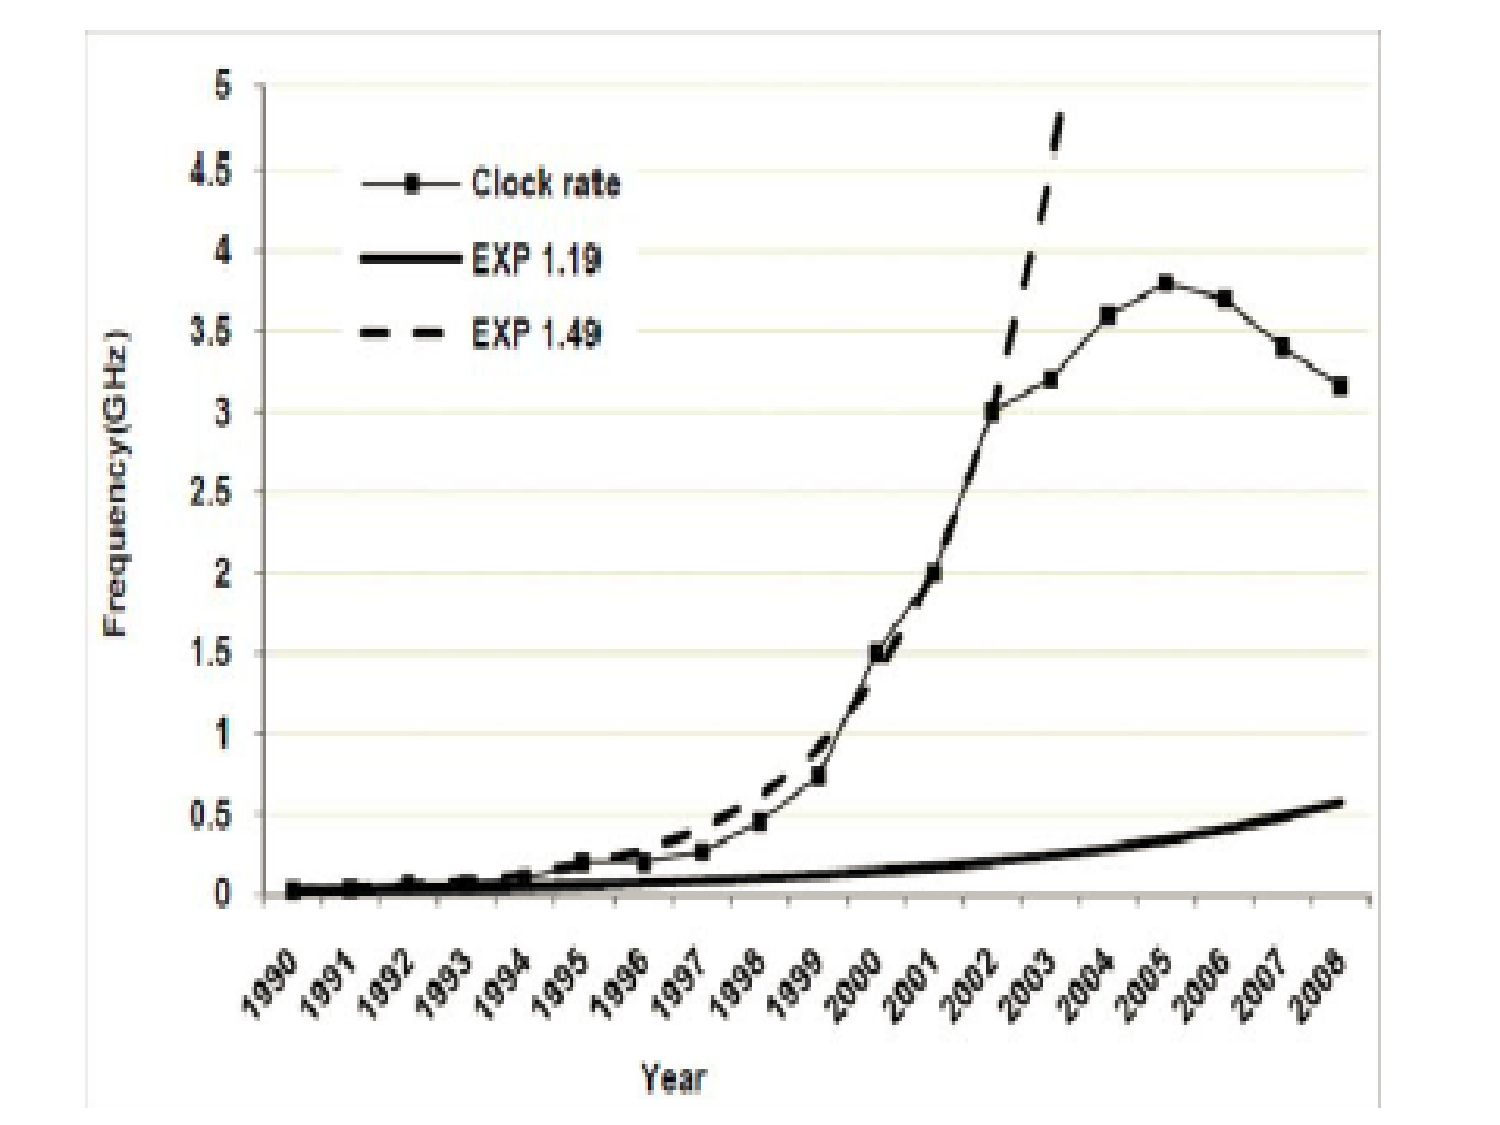
\includegraphics[width=70ex]{Figures/L1/FreqGraph}
\caption{Processor's Clock Frequency (Rate) between 1990-2008.}
%         The $y$ axis is 
%         the frequency; the $x$ axis is the time (years between 
%         1990-2008).}
\label{fig:cpu-freq}
\end{figure} 

Figure~\ref{fig:cpu-freq} shows that historically, the clock
rate (frequency) at which instructions are executed has
increased exponentially between $1990$ to $2004$.

The bolded line in the figure depicts an uniform increase of
$1.19\times$ per year, the dotted line depicts an increase of
$1.49\times$ per year, and the continuous line marked with
black rectangles depicts the actual increase in the clock rate.

The $1.19$ exponential corresponds to technology scaling:
the same hardware is being built on new technology. As silicon
technology improves, the distances shrink (a.k.a., process 
shrinking).  A new technology generation happens about
once every two years, and in each generation transistors'
switching speed increases about $41\%$, which directly
translates to an increase in the clock rate.

Between the years $1990-2002$ the actual increase in clock
rate has matched the $1.49$ exponential: clock rate has doubled 
every $21$ months. If that trend would have continued, we
would have had processors running at $30$GHz by 2008!

The difference between the $1.49$ and $1.19$ exponentials
(up until $2002$) corresponds to improvements in the processor
design. Examples include:
\begin{itemize}
    \item[(1)] Designing very-deep pipelines, consisting of $10-20$ stages.
            Having more stages in the pipeline means that each stage
            is less complex and thus it requires a smaller number of gates 
            per stage. 
            This means that the execution of a stage is quicker, which allows 
            to increase the clock rate. Historically, the number of
            gate delays has dropped by $25\%$ every process generation. 

    \item[(2)] aggressively exploiting instruction-level parallelism (ILP), 
            for example by means of out-of-order, speculative execution, 
            which combine techniques such as register renaming, reordering
            buffers, branch predication, lockup-free caches, speculative 
            memory disambiguation.

    \item[(3)] improvements in circuit design.
\end{itemize}

In $2004$, Intel cancels the design of the Pentium4 $@4$Ghz, and
switches track to multi-core design. This moment constitutes a 
tectonic shift away from the muscled deeply-pipelined uniprocessor.
The clock rate peaked in $2005$ but has mostly stalled since $2002$.

In essence, further increase of the clock rate is unsustainable 
because of a number of reasons: 
\begin{itemize}
\item First, it is unfeasible to build deeper pipelines because it is
difficult to imagine useful stages that can be built from less than
$10$ gates (we have already reached that point).

\item Second, the impact of technology scaling will be blunted in the
future due to wire delays, which do not scale, because the speed 
of wire transmission grows much slower than the switching speed.

\item Finally, and perhaps most importantly, circuits clocked at higher 
rates consume more power, and we have already reached the limits of
power consumption in single-chip microprocessors.
\end{itemize}

However, it is still the case that each process generation---which
roughly happens every two years---offers an additional budget of 
resources, such as transistors, that can be utilized to increase 
performance in other ways than sustaining clock-rate increases.
Figure~\ref{fig:feature-size} shows historical data related to how 
fast the feature size---a unit proportional to the gate length---has 
shrunk over the years and how fast the number of transistors have
grown. In essence, every two years we have a new process generation,
in which the feature size is reduced by about $30\%$ every generation.
The number of transistors also seems to double every two years 
(according to Moore's law), reaching one billion in $2008$.


\begin{figure}
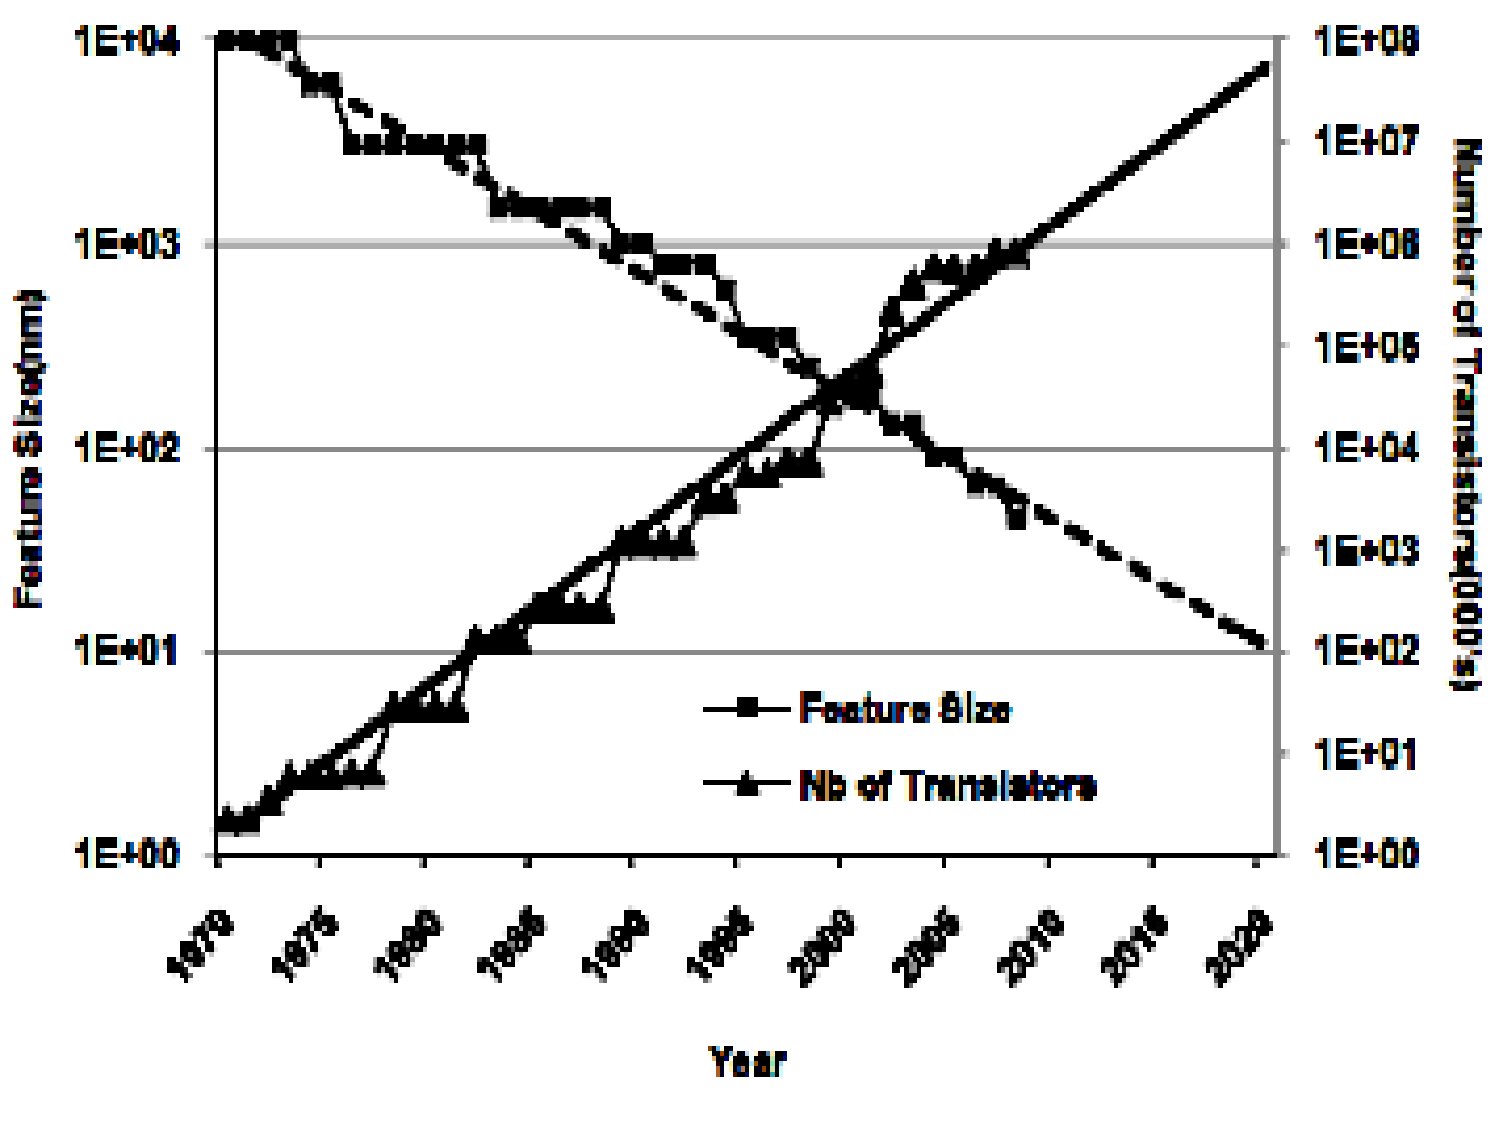
\includegraphics[width=90ex]{Figures/L1/FeatureSize} 
\caption{Historical data and prediction related to the feature-size 
         shrinkage and the number of transistors increase. The feature 
         size is shown by the line starting in the top-left corner;
         the number of transistors is shown in the line starting in 
         the bottom-left corner.}
\label{fig:feature-size}
\end{figure} 

The question thus becomes how to best utilize these hundreds of
billion of transistors in the quest for ever higher performance.
The design of highly-parallel hardware is one (if not the only)
viable direction in this sense. For example the budget of 
transistors can be used to:
\begin{itemize}
    \item enhance the parallelism of the memory system,
    \item to fetch and decode multiple instructions per clock,
    \item to run concurrently multiple hardware threads per 
            core, for example in order to hide the (high) latency
            of the memory system,
    \item to support thousands of cores that run threads in 
            parallel on different cores.
\end{itemize}

\subsection{Memory Wall! Which Memory Wall?}

The term ``memory wall'' was coined to denoted the seemingly
ever-growing gap between the processor and memory speed. This
wall is important because no matter how fast the processor is, 
it still needs to wait for the memory system to deliver the 
data to be processed. 

The historical trends related to memory have been that DRAM density 
increases $4\times$ every three years, but DRAM speed increases
only $7\%$ every year. This in comparison to the processor speed
increasing for a long time by $50\%$ per year.

\begin{figure}
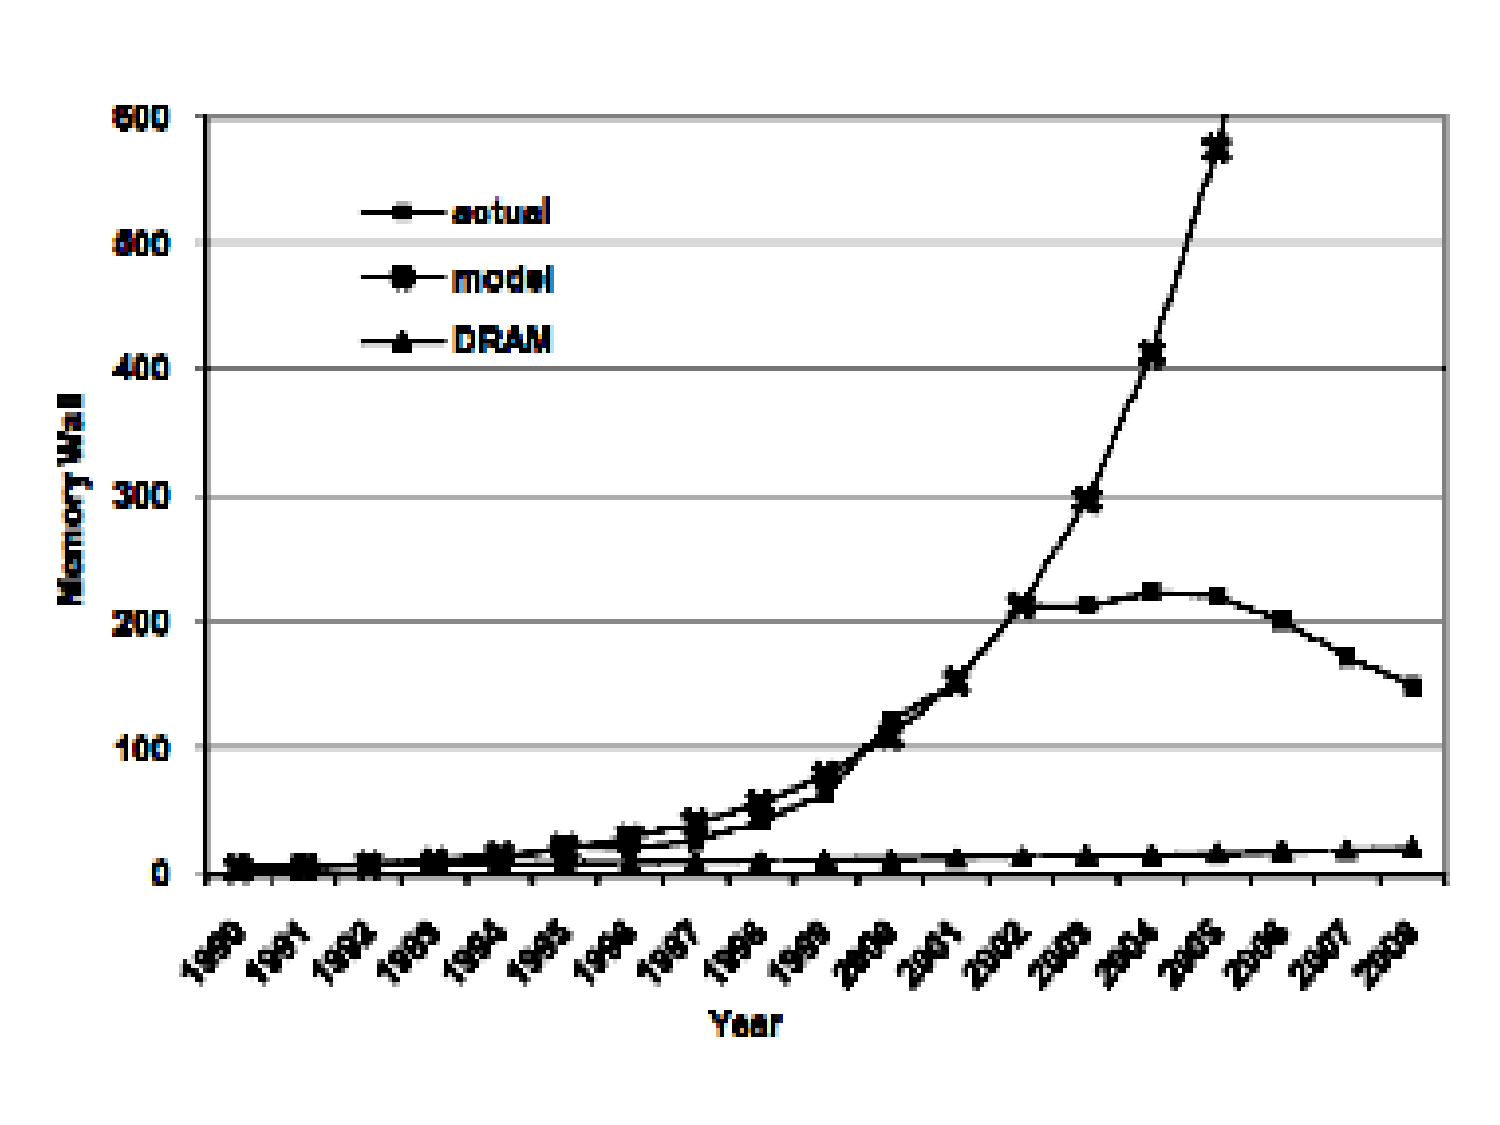
\includegraphics[width=90ex]{Figures/L1/MemWall}
\caption{Historical data related to the memory wall.}
\label{fig:mem-wall}
\end{figure} 

Figure~\ref{fig:mem-wall} shows the historical data related to
the memory wall, which is defined as the ratio between the memory
cycle and the processor cycle: In $1990$, the memory wall was about
$4$, i.e., the processor was running at about $25$MHz, while the 
memory cycle took about $150$ nanoseconds. (Since $1$Hz is $1$ 
cycle/sec, then the processor cycle was about $40$ nanoseconds.)

The memory wall has grown exponentially until $2002$, when it
reached $200$, and the perception was that the memory wall was 
going to last/grow forever.   However, it has stopped growing 
and actually has declined since $2004$ because the clock rate 
of the uniprocessor could not be increased anymore, while the 
DRAM speed still grows, albeit slower.   

As such, the advent of multi- and many-core systems have rendered 
the memory wall obsolete, but have introduced instead a bandwidth wall.
This is because nowadays, the memory subsystem needs to efficiently
feed cores that execute threads in parallel, which means that the
memory system has to be capable of delivering multiple data in 
the same time, which is measured by bandwidth.

%Unrelated, if the trend in DRAM-density increases continues 
%($4\times$ every three years), the figure predicts that DRAM memory 
%will reach one terabit by $2021$, which is still possible to happen.

\subsection{Technological Constraints}

In the past, the main trade-off related to architecture 
design has been between cost (area) and time (performance).
%
Today, the architectural design is challenged by several 
technological limits, such as power, wire delays, reliability,
complexity of design.  We will briefly examined each of them
in the following (sub)sections, and would conclude that 
parallel architectures seem to address well all these 
constraints.

\subsubsection{Power}
$\mbox{ }\\$
The major new constraint is power consumption, which is the sum of
dynamic and static powers:
\[ \mbox{\tt Total Power} ~=~ P_{dynamic} ~+~ P_{static}
\]
The dynamic power is consumed every time a gate is switching states,
i.e., from $0$ to $1$ or from $1$ to $0$, hence it is mostly dissipated 
in processors. It can be computed by the formula:
\[
P_{dynamic} ~=~ \alpha ~C ~V^2 ~f
\]
where $V$ denotes the supply voltage, $f$ denotes the clock rate, 
$T$ denotes the temperature, and $\alpha$ denotes the activity factor
(i.e., $\alpha f$ is the rate at which the gates switch).
%
In a given circuit, an increase in frequency requires a proportional
increase in the supply voltage as well, and a decrease in frequency
allows similarly to reduce the supply voltage. It follows that the
dynamic power consumed is roughly proportional to the cubic power
of the frequency, i.e., $P_{dynamic} \sim f^3$. 
%
As such, dynamic power consumption clearly favors parallel processing 
over increasing the clock rate of the uniprocessor. For example, 
increasing the frequency by a factor of $4\times$ consumes 
$4^3 = 64\times$ more dynamic power, but replicating a uniprocessor 
running at the original frequency $4$ times consumes only 
$4\times$ more dynamic power.
 


The static (leakage) power is dissipated in all circuits, at all times,
no matter of frequency and whether the circuit switches or not. 
In practice, it is dominated by cache leakage. It can be computed
with the formula:
\[
P_{static} ~=~ V ~I_{sub} ~\sim~ V ~e^{-k V_T / T}
\]
where $V_T$ denotes the threshold voltage---the voltage at which
a transistor switches off.  One can observe that the leakage power
increases exponentially as $V_T$ is reduced and as $T$ is increased.

The leakage power was negligible $15$ years ago, but since the feature 
size and the threshold voltage decreases with every process generation,
the leakage is getting worse. Currently, the leakage power has overtaken
dynamic power as the major source of dissipation. 

\subsubsection{Reliability}
$\mbox{ }\\$
Hardware errors/failures can be classified into several categories:
\begin{itemize}
    \item {\bf Transient Failures (Soft Errors).} The charge stored
        in a transistor is $Q = C ~ V$, where $C$ is the capacitance
and $V$ is the supply voltage. In every process generation the supply
voltage is reduced in order to maintain the electrical field at a 
constant strength. Thus $Q$ is considerable reduced at every process
generation, which results in every bit of storage in caches and 
processors being more prone to flip bits due to various corruption
sources, such as cosmic rays, alpha particles radiating from
the packaging material, electrical noise. In essence, the device
is operational, but the data has been partly corrupted. To protect
against such faults, DRAM/SRAM provide some form of error detection 
and correction capabilities.

    \item {\bf Intermittent/Temporary Failures} occur due to environmental
    variations on the chip, such as high temperature (hot spots). 
    In order for the device to return to correct behavior, the cause of
    the errors needs to be removed; for example the device should be 
    switched off for a while, so that the temperature drops. It follows
    that temporary failures last longer than transient failures, but
    they still allow to continue execution (by temporarily switching 
    off the faulty device).

    \item {\bf Permanent Failures} result in permanent damage to the device,
    which will never function properly ever again, and thus the device must 
    be isolated and replaced by a spare one.

\end{itemize}  

Chip mutiprocessors promote better reliability than uniprocessor systems:
For example, threads can be used to redundantly perform the same computation,
and a voting mechanism can be employed to decide the correct answer, and
to temporarily disable a core/resource. Similarly, faulty cores can be
detected and disabled automatically, while the remaining system remains
functional, albeit at a reduced capacity. This allows a natural failsafe
degradation of the system. 

\subsubsection{Wire Delays}
$\mbox{ }\\$
Each process generation shrinks distances, thus enhancing
miniaturization. The consequence is that transistors switch faster,
but the propagation of signals on wire does not keep pace with this
scaling.

To understand why this happens we take a look at the underlying 
physics. The propagation delay on a wire is proportional with the 
product between its resistance and capacitance $\sim R C$. 
The resistance, at its turn, is proportional with the ratio between 
the length and the cross-section area of the wire, i.e., 
$R \sim L / CS_{area}$.
The length of the wire shrinks with every process generation due 
to miniaturization; that is good! The problem however is that
the cross-section area shrinks as well due to the same reason,
which annuls much of the length-shrinking benefits.

The impact of wire delays also favors multiprocessors, because
communication traffic is hierarchical: most communication is 
local, while inter-core communication only happens occasionally.

\subsubsection{Design Complexity}
$\mbox{ }\\$
Design verification has become the dominant cost of chip
development today, and thus constitutes a major design constraint.
The principal reason is that chip density increases much faster 
than the productivity of verification engineers. Much like in
the case of software, this is due to the lack of new, high-level, 
productivity-oriented tools that also run fast.  Verification
is required at several levels of hardware design, such as:
\begin{itemize}
    \item at the gate and register-transfer language level: 
            verifying that the logic is correct,
    \item at the core level: verifying the correctness of 
            forwarding and memory-disambiguation protocols,
    \item at multicore level: verifying the cache-coherency
            and memory-consistency protocols.
\end{itemize}

To some extent, these verification difficulties have resulted in
dedicating the vast majority of chip resources to storage, simply
because it is trivial to increase the size of caches, store/reorder 
buffers, load/store/fetch queues, etc., without compromising the
safety of the design.

The design complexity trend also favors multiprocessors, as it is 
much easier to replicate the same structure multiple times than 
it is to design a large and complex system (or to bring improvements 
to one such). Similar to the case of storage, scaling up the
number of cores of a multiprocessor should not raise major
problems from a design perspective because, for example, 
any reasonable design of the cache-coherency infrastructure
should be parametric in the number of cores. 

\subsubsection{CMOS Meets Quantum Physics}
$\mbox{ }\\$
CMOS\footnote{
    Complementary metal-oxide semiconductor, abbreviated as CMOS,
    is the (current) technology used for constructing integrating 
    circuits. 
} is rapidly reaching the limits of miniaturization: if the current
trend continues, the feature size---defined as half the distance
between two metal wires---will be less than $10$ nanometers 
by year $2020$. This means that the gate length, which is about 
half the feature size, would be in the range of $5$ nanometers.

The radius of the atom is between $0.1$ and $0.2$ nanometers,
and is not affected at all by the miniaturization trends.
%
In essence, the gate length is quickly reaching the range of
atomic distances, which are governed by quantum physics, where
binary logic is replaced with probabilistic states.

While quantum computers are an area of active research, 
it is probably safe to say that commodity quantum hardware is 
not yet quite visible at the horizon. Until that time comes, 
the ever increase in compute power will be achieved by means 
of parallel architectures, such as (clusters of) many cores.
And even if/when quantum hardware will emerge as a viable 
technology, it is also clear that quantum software will be 
massively parallel by nature, so that at least the principles 
of parallel programming will remain of interest.

\newpage

\section{List Homomorphism (LH)}
\label{sec:ListHom}

The goal of the software track of PMPH is to teach the student 
how to ``think parallel''. To achieve this goal we start by
introducing in this section a very simple programming model, 
which utilizes only flat \lstinline{map}-\lstinline{reduce} 
operators, and which is rooted in the mathematical structure 
of list homomorphisms.

\subsection{Math Preliminaries: Monoid and Homomorphism}

This subsection briefly recalls the mathematical structures of
monoid and homomorphism.

A monoid is a set tupled with an associative binary operator, which
accepts an identity element within the set, and a group is a monoid
in which any element is invertible. In formal notation:

\begin{mydef}[Monoid]\label{MonoidDef}
$\mbox{ }$\\
Assume a set $S$ and a binary operator $\odot : S \times S \rightarrow S$.\\
\emph{$(S, \odot)$ is called a monoid} if it satisfies the following two axioms:\\
\emph{(1) Associativity:} $\forall x,y,z\in S$ we have 
    $(x \odot y) \odot z \equiv x \odot (y \odot z)$ and\\
\emph{(2) Identity Element:} $\exists e \in S$ such that $\forall a \in S$, %we have
    $e \odot a \equiv a \odot e \equiv a$.\\\medskip
\end{mydef}

\begin{mydef}[Group]\label{GroupDef}
$\mbox{ }$\\
$(S,\odot)$ is called a group if it is a monoid satisfying the additional
property that any element is  invertible:\\ 
    $\forall a, ~\exists a^{-1}$ such that 
    $a\odot a^{-1}\equiv a^{-1}\odot a\equiv e$.
\end{mydef}

For example, 
\begin{itemize}
    \item $(\mathbb{Z},+)$ denotes the monoid formed by the set of (signed) 
            integers with the addition operation, which has $0$ as neutral
            element. $(\mathbb{Z},+)$ is also a group because any integer
            $i$ has an inverse $-i$, which also belongs to $\mathbb{Z}$. 
            is a group with neutral element $0$.
    \item $(\mathbb{N},+)$ denotes the monoid of natural numbers with
            addition, which has $0$ as neutral element. $(\mathbb{N},+)$  
            is not a group because for example $1$ does not have an 
            inverse in $\mathbb{N}$.
    \item $(\mathbb{Z},\times)$ is the monoid of integers with multiplication,
            which has $1$ as neutral element. $(\mathbb{Z},\times)$ is not
            a group because for example $2$ is not invertible in $\mathbb{Z}$.
            ($\frac{1}{2} \not\in \mathbb{Z}$)
    \item $(\mathbb{L}_T,++)$, is the monoid formed by the set of lists of 
            elements of some type $T$ ($\mathbb{L}_T$), together with the
            list concatenation operator ($++$), which has the empty list
            ($[]$) as neutral element.   $(\mathbb{L}_T,++)$ is obviously
            not a group.
\end{itemize}

A monoid homomorphism is a function between two monoids, such that 
operations on one monoid can be directly mapped into operations on
the second monoid. In formal notation:  

\begin{mydef}[Monoid Homomorphism]\label{HomDef}
$\mbox{ }$\\
\emph{A monoid homomorphism} from monoid $(S,\oplus)$ to monoid $(T,\odot)$
is a function $h : S \rightarrow T$ such that $\forall u, v\in S$,
\emph{$h(u\oplus v) \equiv h(u)\odot h(v)$}.
\end{mydef}


\subsection{The Shape of a List-Homomorphic Function/Implementation}

Throughout this chapter, we will work with finite lists,
albeit the gained insight will carry over to arrays, which
is the main datatype promoting efficient execution on 
modern hardware. We recall that $(\mathbb{L}_T,++)$ is
a monoid:
\begin{itemize}
    \item {\tt ++} denotes list concatenation, for example\\
    {\tt [1, 2, 3] ++ [4, 5, 6, 7] $\equiv$ [1, 2, 3, 4, 5, 6, 7]}
    \item {\tt []} denotes the empty list, which is the neutral 
          element for concatenation:\\ 
            $\forall$ list {\tt x}, we have that 
            {\tt [] ++ x $\equiv$ x ++ [] $\equiv$ x}
\end{itemize}

We will use the term \emph{list-homomorphic function} (LHF)
to denote a function, which accepts an implementation (LHI)
that uses a certain form of divide and conquer programming, 
as defined below.
 
\begin{mydef}[List-Homomorphic Function/Implementation LHF/LHI]\label{LH-FI-Def}
$\mbox{ }$\\
A LHF function $h$ is a (mathematical) function that can be implemented as: 
\begin{lstlisting}[mathescape=true]
h( [ ] )   = e
h( [x] )   = f(x)
h( x ++ y) = h(x) $\odot$ h(y)
\end{lstlisting}
%and which always computes the same result no matter on how 
%the input list is partitioned into {\tt x ++ y}.
\end{mydef}\vspace{-2ex}

In simple words a LH implementation consists of:
\begin{itemize}
    \item[(1)] A divide-and-conquer case 
            {\tt h( x ++ y) = h(x) $\odot$ h(y)},
            which allows to partition the input list {\tt z} 
            into any two sublists {\tt x} and {\tt y} such that
            {\tt z = x ++ y} and the implementation
            applies recursively {\tt h} to the sublists and 
            combines the results with the operator $\odot$.   
            We draw attention to the following important observations:
        \begin{itemize}
            \item[(a)] in order for $h$ to be well defined as a mathematical 
            function (i.e., for the implementation to be useful in practice), 
            $h$ needs to compute the same result no matter of how the input 
            list is partitioned into {\tt x} and {\tt y}. This is an implicit 
            assumption.

            \item[(b)] {\tt h( x ++ y) = h(x) $\odot$ h(y)} essentially
            defines a homomorphism between the monoid $(\mathbb{L}_T,++)$ 
            and another monoid $(Img(h),\odot)$ whose set is the
            image\footnote{
                The image of a function $f : A \rightarrow B$ is the
                subset of $B$ covered by the application of $f$ to
                all elements of $A$.
            } of {\tt h} and its binary operator is $\odot$.
            One remaining question is: ``who is the neutral element of 
            $(Img(h),\odot)$?''
        \end{itemize}

    \item[(2)] Two base cases corresponding to {\tt h} being applied to 
                the empty list and to a list formed by exactly one element:
        \begin{itemize}

            \item[(a)] {\tt e} is the implementation of the
                empty-list case, i.e., {\tt h( [ ] ) = e} and  
                it is actually and provably the neutral element of $(Img(h),\odot)$.
            \item[(b)] the other base case is implemented as
                the application of a function {\tt f} to the
                (single) element of the list.
        \end{itemize}
\end{itemize}

The LHI implementation is utterly unsuitable to being mapped efficiently
to modern highly-parallel hardware, for example because GPUs\footnote{
We use GPU as the abbreviation for general-purpose graphical processing
units.} do not support recursion. However, we remark that the function 
{\tt f}, the binary operator $\odot$ and the neutral element {\tt e} 
are explicitly provided by the LHI and they will allow us later to 
straightforwardly translate this LHI to another implementation which 
can be efficiently mapped on GPU hardware.

The following theorem summarizes our previous observations:
\begin{mytheo}[LHF is a Mathematical Homomorphism]\label{LHF-as-Hom}
$\mbox{ }$\\
A list-homomorphic function (which computes the same result
regardless of how the list is partitioned):
\begin{lstlisting}[mathescape=true]
h( [ ] )   = e
h( [x] )   = f(x)
h( x ++ y) = h(x) $\odot$ h(y)
\end{lstlisting}\vspace{-2ex}
is a mathematical homomorphism from $(\mathbb{L}_T,++)$ to $(Img(h),\odot)$.\\
In particular $(Img(h),\odot)$ must be a monoid with neutral element {\tt e},
which also means that $\odot$ must be associative.\smallskip

The reverse also (trivially) holds: if {\tt h} is a homomorphism between
$(\mathbb{L}_T,++)$ and some monoid $(M,\odot)$ then it accepts a LHI
(as above).\\
\emph{The proof} is left as an exercise. 
\end{mytheo}

\subsection{Examples of List-Homomorphic Implementations}
\label{subsec:LH-egs}

We have discussed so far list homomorphism at a rather abstract
level. This section aims at demonstrating that list-homomorphism
programming is actually quite natural (when it fits) by examining 
several simple code examples. The examples use a notation that 
somewhat resembles Haskell, for example
\begin{itemize}
    \item  greeks such as $\alpha$ denote arbitrary types (type variable),
      and $[\alpha]$ denotes the type of a list whose elements are
      of type $\alpha$,
       
    \item \lstinline{f a b} applies the function \lstinline{f} to two arguments 
      \lstinline{a} and \lstinline{b}, 

    \item \lstinline{&&}, \lstinline{||} correspond to logical and, or operators. 
\end{itemize}

We discuss the following examples:
\begin{itemize}
\item[len:] The first example corresponds to computing the
                length of a list, i.e., 
                {\tt len : $[\alpha] ~\rightarrow$ Int}.
                %The LHI could be:
\begin{lstlisting}[mathescape=true]
len [ ] = 0
len [x] = one x -- where one x = 1
len (x ++ y) = (len x) + (len y)
\end{lstlisting}\vspace{-2ex}
            The first base case says that an empty list has size $0$.
            The second base case says that a list containing exactly
            one element has size $1$; however the LHI form requires
            to call a function on the list's single element, so we
            have defined the function \lstinline{one} to always return $1$
            no matter the argument.
            Finally, the divide-and-conquer case says that if we
            partition the input list into two sublists then the length
            of the initial list is the sum of the lengths of the
            two sublists.\medskip

\item[all$_p$:] The second example corresponds to the function {\tt all$_p$}
            that checks whether some predicate {\tt p : $\alpha ~\rightarrow$ Bool}
            satisfies (holds on) all elements of an input list:
\begin{lstlisting}[mathescape=true]
all$_p$ [ ]      = true
all$_p$ [x]      = p x
all$_p$ (x ++ y) = (all$_p$ x) && (all$_p$ y)   
\end{lstlisting}\vspace{-2ex}
            The base cases say that an empty list satisfies the
            predicate (why?) and that a list containing exactly
            one element satisfies the predicate if and only if
            the element satisfies the predicate (obviously). 
            The recursive, divide and conquer case says that
            a predicate satisfies a list (\lstinline{z = x ++ y}) 
            if and only if it it satisfies both (sub)partitions 
            {\tt x} and {\tt y}.
            The implementation of the empty-list case must be
            \lstinline{true} because this is the neutral element of
            the monoid form by the two-element set 
            {\tt $\{$true, false$\}$} and the logical-and operator (\lstinline{&&}).
            Further intuitive confirmation is given by the fact
            that if {\tt all$_p$ []} is chosen \lstinline{false}
            then the the function {\tt all$_p$} is ill-defined,
            in that it can generate two different results for the same
            input. For example, assume \lstinline{p x = x > 3}. Then 
            {\tt all$_p$ [5, 6]} should result in \lstinline{true}
            because all its elements are greater than three. However,
            the following legal derivation produces \lstinline{false}:
\begin{lstlisting}[mathescape=true]
all$_p$ [5, 6] $\equiv$ all$_p$ ([] ++ [5, 6]) $\equiv$ (all$_p$ []) && (all$_p$ [5, 6]) $\equiv$ 
false && (all$_p$ [5, 6]) $\equiv$ false.
\end{lstlisting}

\item[sum:] The third example corresponds to summing up the (numerical) elements
            of a list. Without further explanation, this can be accomplished
            with the following LHI:
\begin{lstlisting}[mathescape=true]
sum [ ]      = 0
sum [x]      = id x -- where id x = x
sum (x ++ y) = (sum x) + (sum y)
\end{lstlisting}\vspace{-2ex}

\item[fld:] The fourth example corresponds to the function that adds two
            to every (numeric) element of a list and then multiplies the results.
            In F\# this can be expressed as\\ 
            \lstinline{fold (\acc x -> acc * (x+2)) 1 mylist}\\
            Without further ado, this can be accomplished with the following LHI:
\begin{lstlisting}[mathescape=true]
fld [ ]   = 1
fld [x]   = plus2 x -- where plus2 x = x + 2
fld (x ++ y) = (fld x) * (fld y)
\end{lstlisting}\vspace{-2ex}
\end{itemize} 


\subsection{Map, Reduce and List Homomorphism Theorems}

This section (i) starts by introducing two of the (three) important 
basic blocks that lay the foundation of data-parallel programming
(\lstinline{map} and \lstinline{reduce}),
then (ii) presents the first theorem of list homomorphism, which 
basically gives a straightforward way of translating a LHI into
a semantically-equivalent \lstinline{map-reduce} implementation,
and (iii) it concludes by presenting several other theorems that
can be seen as simple re-write rules that allow to optimize the 
program in various ways.

It is perhaps important to notice that while the discussion refers
to lists, this is only to preserve consistency with the
list-homomorphism presentation. List is an implicitly sequential 
datatype; whenever we mention lists from now on, the reader
should think arrays, at least in what parallel execution is concerned. 

The first basic-block of data parallel programming is the 
\lstinline{map} second-order operator, which takes as argument 
an unary function and a list of elements, and produces a list 
of the same length as the original one by applying the function 
argument to each element of the input list.  
The type and semantics of \lstinline{map} are presented below:
\begin{lstlisting}[mathescape=true]
map : $(\alpha \rightarrow \beta) ~\rightarrow ~[\alpha] ~\rightarrow~ [\beta]$
map f [x$_1,\ldots$x$_n$] = [f x$_1$,$\ldots$, f x$_n$]
\end{lstlisting}\vspace{-2ex}

Please note that, assuming a pure-functional language and replacing
lists with arrays, \lstinline{map} has implicitly parallel semantics, 
because the computation corresponding to some element {\tt x$_i$}
of the array is completely independent of the computations of all
other elements of the array.


The second basic-block of data parallel programming is the
\lstinline{reduce} second-order operator, which takes as arguments
an \emph{associative} binary operator, the neutral element corresponding
to the monoid defined by the binary operator, and a list of elements.
The result of \lstinline{reduce} is obtained by successively applying 
the operator to all the elements of the array. The type and semantics of 
\lstinline{reduce} are presented below:
\begin{lstlisting}[mathescape=true]
reduce : $(\alpha \rightarrow \alpha \rightarrow \alpha) ~\rightarrow~ \alpha ~\rightarrow~ [\alpha]~ \rightarrow \alpha$
reduce $\odot$ e [x$_1,\ldots$x$_n$] = e $\odot$ x$_1$ $\odot~\ldots~\odot$ x$_n$
\end{lstlisting}\vspace{-2ex}

Unlike \lstinline{map}, the parallel semantics of \lstinline{reduce}
is not straightforward to see. We demonstrate it in 
\cref{fig:reduction-tree}: assuming an infinite number of
processors, the parallel computation of \lstinline{reduce} is 
performed by means of a reduction tree, which performs sequentially
a number of {\tt log(n)} parallel operations, where we have denoted
by {\tt n} the length of the input array. 


\begin{figure}
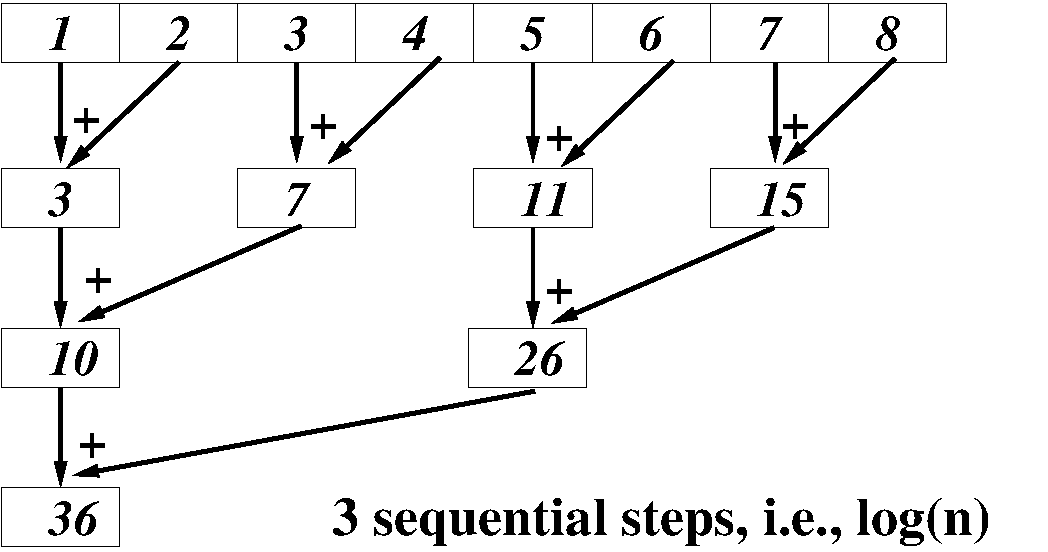
\includegraphics[width=70ex]{Figures/L1/ReduceEg.pdf}
\caption{Parallel execution of \lstinline{reduce} requires
        a sequence of \lstinline{log(n)} parallel operations
        ({\tt n} is the array length).}
\label{fig:reduction-tree}
\end{figure} 

It is perhaps important to stress (again) that $\odot$ \emph{\bf must be 
associative}:
\begin{itemize}
    \item In parenthesis, that is why we did not bother to put 
the parenthesis that would specify the execution order, 
but the commonly-used sequential implementation of \lstinline{reduce} 
accumulates to the left, i.e., 
{\tt ((e $\odot$ x$_1$) $\odot~\ldots~\odot$ x$_n$)}.

    \item More importantly, if $\odot$ is not associative then the 
    sequential and parallel execution of \lstinline{reduce} will likely
    give different results. For example,  assume the list \lstinline{[1,2,3,4]}
    which is reduced with the non-associative operator {\tt acc $\odot$ x = acc + 2*x}.
    Even ignoring the neutral element, sequential execution will 
    result in {\tt (((1 $\odot$ 2) $\odot$ 3) $\odot$ 4) = 19}
    and parallel execution will result in 
    {\tt (1 $\odot$ 2) $\odot$ (3 $\odot$ 4) = 5 $\odot$ 11 = 27},
    according to the execution patterns of the reduction tree shown
    in \cref{fig:reduction-tree}.
    
    \item It should be clear now that \lstinline{reduce} is different
        that \lstinline{fold} (from F\#). This can be seen from
        the type of {\tt fold : ($(\beta \rightarrow \alpha \rightarrow \beta) ~\rightarrow~ \beta ~\rightarrow~ [\alpha]~ \rightarrow \beta$}; in particular it does not make sense
        to talk about the associativity of \lstinline{fold}'s operator
        because of the wrong type---associativity makes sense on
        binary operators whose arguments and result have the same type.
        Moreover, even when the type happens to be correct, as in the
        previously-discussed case, we have still seen that \lstinline{fold} 
        is not a parallel operator because it does not require associativity.
        In particular \lstinline{fold (\acc x -> acc + 2*x) 0 lst}
        can be parallelized by re-writing it as a \lstinline{map-reduce} 
        composition: \lstinline{reduce (+) 0 (map (+2) lst)}!

    \item In practice forgetting that the \lstinline{reduce} operator
             must be associative---i.e., using \lstinline{reduce} with
             non-associative operators---is one of the main generators 
             of difficult-to-find bugs.
\end{itemize}

Similarly, remember that {\tt e} must be the neutral element of the 
monoid defined by $\odot$---hence reducing an empty list results in 
{\tt e}, and {\tt e} can be safely omitted from the computation if 
the list is not empty (because by the definition of the neutral 
element, we have that {\tt e $\odot$ x $\equiv$ x, $\forall$ x}).

\subsubsection{First List-Homomorphism Theorem}
$\mbox{ }$\\

The first LH theorem~\cite{ThirdLHTh} basically gives a 
straightforward way of rewriting a LHI as a \lstinline{map-reduce} 
composition, as stated in the theorem below, which uses $\circ$ 
to denote the function-composition operator.

\begin{mytheo}[1$^{st}$ LH Theorem]\label{1st-LH-TH}
$\mbox{ }$\\
A list-homomorphic implementation defined as:
\begin{lstlisting}[mathescape=true]
h( [ ] )   = e
h( [x] )   = f(x)
h( x ++ y) = h(x) $\odot$ h(y)
\end{lstlisting}\vspace{-2ex}
is semantically equivalent with
(\lstinline{reduce}$~\odot~$\lstinline{e})$~~\circ~~$(\lstinline{map f}),
or in complete code:
\begin{lstlisting}[mathescape=true]
h z $\equiv$ reduce $\odot$ e (map f z)
\end{lstlisting}\vspace{-2ex}
\end{mytheo}

\cref{1st-LH-TH} also provides the theoretical argumentation of why the
\lstinline{reduce} operator must be associative: if $h$ is a list
homomorphism, then $(Img(h),\odot)$ must be a monoid, and by definition,
a monoid requires its operator $\odot$ to be associative.

Applying \cref{1st-LH-TH} to the LHI discussed in \cref{subsec:LH-egs}
results in the following \lstinline{map-reduce} implementations:
\begin{itemize}
    \item \lstinline{len z} $\equiv$ \lstinline{reduce (+) 0 (map one z)}
    \item {\tt all$_p$ z $\equiv$} \lstinline{reduce (&&) true (map p z)}
    \item \lstinline{sum z} $\equiv$ \lstinline{reduce (+) 0 (map id z)} $\equiv$ \lstinline{reduce (+) 0 z}
    \item \lstinline{fld z} $\equiv$ \lstinline{reduce (*) 1 (map plus2 z)}
\end{itemize}

We have thus started from an arguably natural program specification rooted 
in the mathematical theory of list homomorphisms, and we have translated
that into an implementation in which parallelism is made explicit by
\lstinline{map-reduce} operators and which can be straightforwardly
mapped to modern parallel architectures. We discuss simple program
optimizations next.

\subsubsection{Other List-Homomorphism Lemmas}

\begin{mytheo}[LH Promotion Lemmas]\label{LH-PROMS}
$\mbox{ }$\\
Given unary functions \lstinline{f} and \lstinline{f}, and an 
associative binary operator $\odot$ with neutral element {\tt e$_{\odot}$}
then the following three identities hold, where $\circ$ denotes 
function composition:\\
\begin{lstlisting}[mathescape=true]
1. (map f) $\circ$ (map g) $\equiv$ map (f $\circ$ g)
2. (map f) $\circ$ (reduce (++) []) $\equiv$ (reduce (++) []) $\circ$ (map (map f))
3. (reduce ($\odot$) e$_{\odot}$) $\circ$ (reduce (++) []) $\equiv$
                         (reduce ($\odot$) e$_\odot$) $\circ$ (map (reduce ($\odot$) e$_{\odot}$)) 
\end{lstlisting}
If you are unfamiliar with the functional notation for composition, 
the identities can be written in full as:\\
\begin{lstlisting}[mathescape=true]
1. map f (map g zs) $\equiv$ map ($\lambda$ z $\rightarrow$ f (g z)) zs
2. map f (reduce (++) [] zs) $\equiv$ reduce (++) [] (map ($\lambda$z$\rightarrow$map f z) zs)
3. reduce ($\odot$) e$_{\odot}$ (reduce (++) [] zs) $\equiv$ 
                        reduce $\odot$ e$_\odot$ (map ($\lambda$ z $\rightarrow$ reduce $\odot$ e$_{\odot}$ z)) 
\end{lstlisting}\vspace{-2ex}
\end{mytheo}

The identities can be seen as re-write rules that can be used
to optimize the program in various ways, for example:
\begin{itemize}
    \item[(1)] The first identity is known as the \lstinline{map} fusion/fission
        rule:
        \begin{itemize}
            \item[$\Rightarrow$] Fusion corresponds to applying the transformation 
                    in the forward ($\Rightarrow$) direction, and is 
                    useful for reducing the number of accesses to
                    global memory, which is very slow in comparison
                    with registers. For example, the left-hand side
                    program: \lstinline{let tmp = map g zs in map f tmp}
                    requires to read and write in the first \lstinline{map}
                    each element of arrays {\tt zs} and {\tt tmp}, respectively,
                    followed by reading and writing in the second 
                    \lstinline{map} each element of {\tt tmp} and result
                    arrays, respectively. This counts up to $4$ accesses
                    to global memory per element. The program on the
                    right-hand side: \lstinline{map (}$\lambda$ {\tt z} $\rightarrow$ {\tt f (g z)) zs} 
                    requires reading and writing the input and result arrays
                    only once, thus halving the number of accesses to global
                    memory per element---because the intermediate computation
                    {\tt g z} is hold in registers, not in memory.
            \item[$\Leftarrow$] Fission corresponds to applying the transformation 
                    in the backward ($\Leftarrow$) direction and is useful
                    for enhancing the degree of parallelism that is statically mapped
                    to hardware, in the context of a nested-parallel program.
                    (This will be discussed in detail later on in the context 
                    of the flattening transformation and vectorization.)
        \end{itemize}

    \item[(2,3)] Similar to fusion/fission, the second and third identities can 
                    be used in the forward 
                    direction ($\Rightarrow$) to efficiently sequentialize 
                    the parallelism in excess of what the hardware can support, 
                    and in the backward direction ($\Rightarrow$)  
                    to enhance load balancing and the program's degree of 
                    parallelism that can be statically mapped to hardware.
        \begin{itemize}
            \item[$\Rightarrow$]
                    The second identity can be rewritten as:\\
                    \lstinline{map f} $\Rightarrow$ \lstinline{(reduce (++) [])} $\circ$ \lstinline{(map (map f))} $\circ$ {\tt split$_p$}\\
                    where {\tt split$_p$} denotes the operator that splits a list
                    into $p$ sublists of roughly equal lengths.  Assume the hardware
                    has $p$ cores, and that the input list (array) contains
                    $n$ elements, where $n$ is much larger than $p$. The right-hand side 
                    \lstinline{map f} suggests an execution model that spawns $n$
                    threads---this is suboptimal on many architectures.
                    The translation basically aims to spawn a number of threads
                    equal to the number of cores. This is achieved by splitting
                    the list, then processing sequentially each chunk on one core
                    (by the inner \lstinline{map}), while processing the $p$ chunks 
                    in parallel (by the outer \lstinline{map}), and finally by
                    concatenating the per-core results. Similar thoughts apply to
                    the third identity.   
                    
            \item[$\Leftarrow$] Consider a program similar to the left-hand side
                    of the original identity $2$. Its input is necessarily a list
                    of lists. Assume the input list has $p$ unbalanced sublists, 
                    for example all sublist have $2$ elements, except for the
                    last one which has $n - 2\cdot p - 2$ elements, where 
                    $n$ is big. If executed as suggested by the right-hand side---each
                    core processes a sublist---the parallel execution will be
                    utterly unbalanced because the last core will process many
                    more items than the rest of the cores. If processing an
                    item uniformly takes one unit, then the speedup achieved 
                    by the right-hand side program will be $\frac{n}{n - 2 \cdot p - 2}$
                    which converges to $1$ when $n$ goes to infinity.
                    Instead, one can apply the second identity in the $\Leftarrow$ 
                    direction to flatten parallelism, then one can apply again 
                    the forward direction as in the $\Rightarrow$ bullet above
                    by splitting the concatenated list again into $p$ sublists 
                    of \emph{roughly-equal} lengths. The execution of the resulting
                    program is now load-balanced, each core processing a similar
                    number of elements, resulting in a speedup close(er) to
                    the optimal $p\times$. Similar thoughts apply to the third identity.
        \end{itemize}
\end{itemize}


The final theorem is often used for optimizing the scheduling of 
\lstinline{map-reduce} computations, for example in frameworks such
as OpenMP. The idea is that a \lstinline{map-reduce} composition
can be re-written into a semantically equivalent program that:
\begin{itemize}
    \item splits the input list into $p$ sublists of roughly
            equal length,
    \item applies the original computation to each sublist,
            such the computation of a sublist is performed
            sequentially on a core, but different sublists
            are processed in parallel on different cores, 
    \item applies the original reduction to the per-core
            results.
\end{itemize}
The benefit of such an execution is not only given by
spawning a number of threads equal to the numbers of cores,
thus reducing scheduling and switching-contexts overheads,
but also optimizing the reduction depth. Originally,
the reduction was applied to a list of $n$ elements,
and would require $log(n)$ sequential steps (see reduction
tree in \cref{fig:reduction-tree}). In the
transformed program the final (parallel) reduction
is performed on a list of $p$ elements, requiring only
$log(p)$ sequential steps.

\begin{mytheo}[Optimized Map-Reduce Lemma]\label{Lemma-Map-Red}
Assume {\tt split$_p :: [\alpha] \rightarrow [[\alpha]]$}
distributes a list into $p$ sublists, each containing about 
the same number of elements. Also assume $\odot$ a binary 
associative operator with neutral element {\tt e$_{\odot}$} 
and {\tt f} a unary function. The following identity always holds:
\begin{lstlisting}[mathescape=true]
redomap ($\odot$) f e$_{\odot}$ $\equiv$
(reduce ($\odot$) e$_{\odot}$) $\circ$ (map (redomap ($\odot$) f e$_{\odot}$)) $\circ$ split$_p$
\end{lstlisting}\vspace{-2ex}

where \lstinline{redomap} is defined as
\lstinline{redomap} $\odot$ {\tt f e$_{\odot}$} $\equiv$ \lstinline{(reduce} $\odot$ {\tt e$_{\odot}$)} $\circ$ \lstinline{(map f)}.

\emph{The Proof} is left as an exercise. 
\end{mytheo}

In what the proof of \cref{Lemma-Map-Red} is concerned, the big hint is to first 
observe that\\
\lstinline{(reduce (++) [])} $\circ$  {\tt distr$_p$} results in the identity function,
which is the neutral element for function composition---concatenating the result obtained
by splitting an input list results in the input list. As such we can start
by composing the left-hand side with the identity written as before:\\
\lstinline{redomap} {\tt($\odot$)} {\tt f e$_{\odot}$} $\equiv$ \lstinline{(reduce} {\tt($\odot$)} {\tt e$_{\odot}$)} $\circ$ \lstinline{(map  f)} $\circ$ \lstinline{(reduce (++) [])} $\circ$ {\tt split$_p$} $\equiv~\ldots$\\
and then it takes about three applications of the promotion lemmas of \cref{LH-PROMS} 
to derive the right-hand side of the identity stated by \cref{Lemma-Map-Red}. 

\subsection{Almost/Near Homomorphisms [Gorlatch/Cole]}

The notion of \emph{near homomorphism}~\cite{ColeNearHom} or 
synonymously \emph{almost homomorphism}~\cite{Gorlatch:AntiUnif} 
has been introduced (independently) by Murray Cole and 
Sergei Gorlatch, respectively. 

The simple intuition is that a non-homomorphic function $g$ can 
be sometimes ``lifted'' into a homomorphic one, by computing
a baggage of extra information. If this is possible, then the
result of the original problem can be obtained by projecting
the homomorphic result (e.g., by selecting an element from a tuple).
%$g\mbox{ }=\pi\mbox{ }.\mbox{ }f$

We will demonstrate the near-homomorphism construction on two
interesting problems, which are going to be examined and solved
in the rest of this chapter.

\subsubsection{Maximum-Segment Sum (MSS) Problem}:
$\mbox{ }$\\

The formulation of MSS problem is:\bigskip

\emph{``Given a list of signed integers, find the contiguous segment 
  of the list whose members have the largest sum among all 
  such segments; the result is only the maximal sum, 
  not the segment's members.''}\bigskip

For example, the MSS of \lstinline{[1, -2, 3, 4, -1, 5, -6, 1]}
is \lstinline{11}, and the corresponding maximal segment is 
\lstinline{[3, 4, -1, 5]}.

One can observe that it is impossible to express this problem
directly in a list-homomorphism way---such that the operator 
of the reduction receives two integers as arguments and 
produces an integer, i.e., 
$\odot ~:~ \mbox{\tt int}\rightarrow\mbox{\tt int}\rightarrow\mbox{\tt int}$. 
For example, assume the list has been split as 
$l_1=$\lstinline{[1, -2, 3, 4]} and $l_2=$\lstinline{[-1, 5, -6, 1]}. 
According to the definition of MSS, the human can observe that 
the MSS of sublist $l_1$ is $7$ (corresponds to segment \lstinline{[3,4]}), 
and the MSS of sublist $l_2$ is $5$ (corresponds to segment \lstinline{[5]}).

Having the result of MSS for each sublist summarized only as an
integer prevents us from meaningfully combining the sublists results
into a result that is correct for the whole list. 
For example, with what operator should we combine $7$ and $5$?
Should it be addition, which would result in MSS being $12$,
or should it be the maximal value, which will result in $7$, or what?

Neither give the correct result, which we recall is $11$ for
the given input. 
The reason is that the maximal segment can very well lie across
$l_1$ and $l_2$, i.e., partly in $l_1$ and partly in $l_2$,
but this case cannot be covered by a reduce operator working on
integers---we need to provide the reduce operator with additional
information.

For example, one can reason that it would be useful to maintain
for each (sub)list:
\begin{itemize}
    \item[(mis)] an integer corresponding to the maximal 
        sum across all contiguous segments that starts the 
        list (i.e., those containing the first element);
        we will name this the maximal-initial sum {\tt mss}, 
    \item[(mcs)] and similar for the contiguous segments that 
        ends a list (i.e., those containing the last element);
        we will name this the maximal-concluding sum {\tt mcs}.
        With this extra information one could reason that
        the operator that combines the results of two sublists 
        $l_1$ and $l_2$ should chose the maximal value between 
        the MSS of $l_1$, the MSS of $l_2$, and the maximal
        segment that crosses $l_1$ and $l_2$ (i.e., lies partly 
        in $l_1$ and partly in $l_2$), which is obtained
        by adding the {\tt mcs$_1$} of $l_1$ with the 
        {\tt mis$_2$} of $l_2$.
        (Since we consider only contiguous segments, a crossing 
         segment \emph{will necessarily be} a composition of an
         {\tt mcs} of $l_1$ with an {\tt mis} of $l_2$.)
        It would seem that we have successfully figured out
        how to compute the MSS of two sublists, but this
        computation requires the {\tt mis} and {\tt mcs}
        of the two sublists; how do we compute those?

    \item[(ts)] To compute {\tt mis} and {\tt mcs} we need only
        one extra piece of information: the total sum of a
        sublist, denoted as {\tt ts}. Assume we have the
        results for $l_1$ and $l_2$ and we want to compute
        the {\tt mis} for $l = l_1 \mbox{\tt++} l_2$.
        We can reason that the {\tt mis} of $l$ is the maximal
        value between:
        \begin{itemize}
            \item the {\tt mis$_1$} of $l_1$, because the initial
            segments of $l_1$ are also initial segments of $l$, and
            \item {\tt ts$_1$ + mis$_2$}, because the maximal
            initial segment of $l$ may span across its two sublists---in
            this case, by definition of initial segment, it necessarily 
            needs to include the whole sublist $l_1$ and the maximal 
            initial segment of $l_2$.
        \end{itemize}
        Similar considerations apply to computing the {\tt mcs} of
        of $l$. 
\end{itemize}

We have applied above a list-homomorphic (divide-and-conquer) type of
reasoning, in that we have derived what the reduce operator should be
in terms of thinking how to combine the results of two sublists into
the result of a list. We are now ready to write directly the
\lstinline{map-reduce} (obtained by applying \cref{1st-LH-TH}):

\begin{lstlisting}[mathescape=true]
-- $\odot$ : (int,int,int,int) $\rightarrow$ (int,int,int,int) $\rightarrow$ (int,int,int,int)
(mss$_1$, mis$_1$, mcs$_1$, ts$_1$) $\odot$ (mss$_2$, mis$_2$, mcs$_2$, ts$_2$) =
    let mss = max (max mss$_1$ mss$_2$) (mcs$_1$+mis$_2$)
    let mis = max mis$_1$ (ts$_1$ + mis$_2$)
    let mcs = max mcs$_2$ (ts$_2$ + mcs$_1$)
    let ts  = ts$_1$ + ts$_2$
    (mss, mis, mcs, ts)

-- f : int $\rightarrow$ (int,int,int,int)
let f x = (max x 0, max x 0, max x 0, x)

-- $\pi_1$ : (int,int,int,int) $\rightarrow$ int
let $\pi_1$ (x, _, _, _) = x

-- maxSgmSum : [int] $\rightarrow$ int
let maxSgmSum xs = 
    let exp_xs  = map f xs
    let exp_res = reduce ($\odot$) (0,0,0,0) exp_xs
    $\pi_1$ exp_res 
\end{lstlisting}\vspace{-2ex}

In essence, the implementation of MSS, denoted {\tt maxSgmSum} 
has three main steps:
\begin{itemize}
    \item[\bf{map:}] first each element of the input array {\tt xs} is lifted
            to a quad-tuple, by applying {\tt f}---this allows to compute a
            larger baggage of information, i.e., {\tt mis, mcs, ts};
    \item[\bf{reduce:}] then the result is reduced with the operator $\odot$
            as explained above;
    \item[\bf{project:}] finally, we select (project) the first element of
            the result tuple that contains the information of interest (the MSS)
            and discard the rest.
\end{itemize}

The implementation above diverges a bit from the definition of MSS,
in that the result is always positive---we kept this form in order 
to be consistent with the original paper~\cite{ColeNearHom}.  If
we would like also to compute negative MSS values, we can change
the implementation of {\tt f} to
\lstinline{let f x = (x,x,x,0)} and the neutral element of $\odot$
to {\tt($-\inf, -\inf, -\inf, 0$)}.

\subsubsection{Longest-Satisfying Segment (LSS) Problem}:
$\mbox{ }$\\

LSS denote a class of near-homomorphic problems which requires 
to find the length of the longest (contiguous) segment of a list 
for which some property holds.
For example, we might want to compute:
\begin{itemize}
    \item[{\bf zeros:}] the length of the longest segment of 
            zeros, or 
    \item[{\bf same:}]  the length of the longest segment made 
            from the same number, or 
    \item[{\bf sorted:}] the length of the longest sorted 
            sequence.
\end{itemize}

Please notice however, that it is \emph{not} the case that all 
predicates result in a LSS problem that can be expressed as a
list (near) homomorphism. For example the length of the longest 
sequence whose sum is $0$ is \emph{not} expressible as a list 
homomorphism.

It turns our that if we restrict the predicate to have a certain
shape, than all such predicates allow a list-homomorphic implementation.
The shape of the restricted predicate is:

\begin{lstlisting}[mathescape=true]
p []          = true
p [x]         = ... -- some implementation
p [x, y]      = ... -- some implementation
p (x:y:zs) = (p [x,y]) && (p (y:zs))
-- where && denotes the logical-and operator
-- and : denotes the cons operator, i.e., x : y : z : [] == [x,y,z] 
\end{lstlisting}\vspace{-2ex}

Note that various predicates can be implemented by filling in the 
computation of the base cases when the list contains one and two
elements, respectively.   For example, the predicates for the
three list-homomorphic problems listed above are derived by the
following implementation of the base cases:

\begin{lstlisting}[mathescape=true]
zeros [x]   = (x == 0)           
zeros [x,y] = (zeros [x]) && (zeros [y])

same [x]   = true         
same [x,y] = (x == y)

sorted [x]   = true
sorted [x,y] = (x <= y)
\end{lstlisting}\vspace{-2ex}

Now that we finally defined what a LSS problem is, it remains the reason about
what should be the baggage of extra information that would allow us to lift a 
LSS problem to accept a list-homomorphic implementation. The rational is
somewhat similar to the one for maximal segment sum, but with several additions:

\begin{itemize}
    \item As before, we need to maintain the \emph{length} of the longest 
            initial and concluding satisfying segments, which we denote
            by {\tt lis} and {\tt lcs}, respectively, together with the
            total length of the (sub)list, denoted by {\tt tl}.

    \item When considering the concatenation of the {\tt (lcs$_1$, lis$_2$)} 
            pair---i.e., for the case when the segment of interest spans 
            across the two sublists---it is not guaranteed that the spanning 
            segment satisfies the predicate; this must be explicitly checked! 
            For example, if the elements of some lists $x$ and $y$ are in 
            sorted order, this does not means the the list obtained by 
            concatenating $x$ with $y$ has elements in sorted order: 
            {\tt (sorted l$_1$) \&\& (sorted $l_2$) $\not\Rightarrow$ sorted ($l_1$++$l_2$)}.  
            
    \item To perform the check mentioned above, we need to record the 
            \emph{last} element of {\tt lcs} and the \emph{first} element of {\tt lis}.
            This would allow to compute whether {\tt lcs$_1$} is \emph{connected} 
            to {\tt lis$_2$}, by checking the condition {\tt p [lastx,firsty] == True}.
\end{itemize}

\subsubsection{Exercise: Longest-Satisfying Segment (LSS) Implementation}:
$\mbox{ }$\\

The implementation of the longest-satisfying segment is proposed as an exercise
(first weekly assignment).  You will need to fill in the blanks in the skeleton
code below. You should also implement it in Futhark, run it on the GPU-equipped
machines and report the speedup between the accelerated and CPU-based versions
(obtained by compiling with {\tt futhark-opencl} and {\tt futhark-c}, 
respectively):\bigskip

\begin{lstlisting}[mathescape=true]
(lss$_1$, lis$_1$, lcs$_1$, tl$_1$, frst$_1$, last$_1$) $\odot$
(lss$_2$, lis$_2$, lcs$_2$, tl$_2$, frst$_2$, last$_2$) =
    let connect = ... -- fill in the blanks
    let lss     = ... -- fill in the blanks
    let lis     = ... -- fill in the blanks
    let lcs     = ... -- fill in the blanks
    let tl      = ... -- fill in the blanks
    let frst    = if tl$_1$ == 0 then frst$_2$ else frst$_1$
    let last'   = if tl$_2$ == 0 then last$_1$ else last$_2$
    (lss, lis, lcs, tl, frst, last')

let f x = 
    let xmatch = if (p [x]) then 1 else 0    
    (xmatch, xmatch, xmatch, 1, x, x)

let $\pi_1$ (a, _, _, _, _, _) = a

let lgstSatSgm xs = 
    let exp_xs  = map f xs
    let exp_res = reduce ($\odot$) (0,0,0,0,0,0) exp_xs
    $\pi_1$ exp_res 
\end{lstlisting}\vspace{-2ex}

\subsection{Conclusion}

This section has started by presenting a program specification rooted in
the mathematical structure of list homomorphism, and which corresponds to
an (arguably) natural, divide-and-conquer way of expressing a class of
simple problems.   We have then shown that such a program has an implicitly
parallel semantics because it can be straightforwardly translated into a
semantically-equivalent program written in terms of \lstinline{map-reduce} 
compositions.   

We have drawn attention that the reduce operator must be
associative because the homomorphism theory requires it, and we have
also drawn attention that a {\tt fold} does not always have parallel 
semantics, because not even that its semantics does not require 
its binary operator to be associative, but we cannot even talk about 
it's operator's associativity (wrong type). However, we have seen
that frequently, a {\tt fold} can be rewritten by means of a 
\lstinline{map-reduce} composition. 

Next, we have studied several (promotions) lemmas derived naturally
from the list-homomorphism theory, and we have explained that they can
be seen as re-write rules, and can be used to optimize a program in 
different ways.

Finally, we have examined two classes of problems (MSS and LSS), 
whose (efficient) parallel nature is far from trivial even to understand, 
and we have shown that list-homomorphic 
(divide-and-conquer) reasoning can straightforwardly derive 
efficient parallel implementations for these problems.

The next \cref{sec-nested-par} will introduce several other parallel 
operators that are basic blocks of data-parallel programming, 
such as \lstinline{scan}, and will demonstrate how to reason about 
the efficiency of a parallel program in terms of asymptotic properties 
such as work and depth.
More importantly, it will show that complex programs can be built as
puzzles from a \emph{nested} composition of operators such as 
\lstinline{map}, \lstinline{reduce}, \lstinline{scan}.

Furthermore, \cref{sec:flattening} will give the intuition behind a 
transformation that can automatically rewrite a nested-parallel 
program into a flat-parallel one that can be statically mapped to 
highly-parallel hardware, in a way that preserves the asymptotic 
work-depth properties of the original (nested-parallel) program. 

\newpage
\section{Work-Depth Asymptotic, Nested Parallelism}
\label{sec-nested-par}

This section is organized as follows: 
\begin{itemize}
    \item \cref{subsec:work-depth} introduces and demonstrates 
        how to characterize parallel programs in terms of 
        work and depth complexity. 
            
    \item \cref{subsec:nest-par-app} extends the set of parallel
        operators---with scan, filter, scatter---and demonstrates
        how several parallel programs, such as sparse matrix-vector 
        multiplication, prime number computation, quicksort---can
        be elegantly expressed by nesting parallel constructs, and 
        how their efficiency can be reasoned in terms of their 
        work-depth asymptotic.
\end{itemize}

\subsection{Reasoning in Terms of Work-Depth Asymptotic}
\label{subsec:work-depth}

This section starts by presenting Amdahl's law as a way to
motivate why it is necessary to write programs as if the
hardware provides an infinity number of cores. We then
briefly present a simplified and idealized parallel hardware 
(PRAM) that is used to introduce the notion of work and depth 
complexity of a (nested) parallel program. 

We then argue, by means of Brent's theorem, that the 
work-depth measure is a good approximation of the parallel 
behavior of the program, and we demonstrate how one can 
reason about computing the program's work and the depth 
for the simple case of summing up the elements of an array.

\subsubsection{Amdahl's Law}
\label{subsubsub:amdahl}
$\mbox{ }$\\

\begin{figure}
\vspace{-3ex}
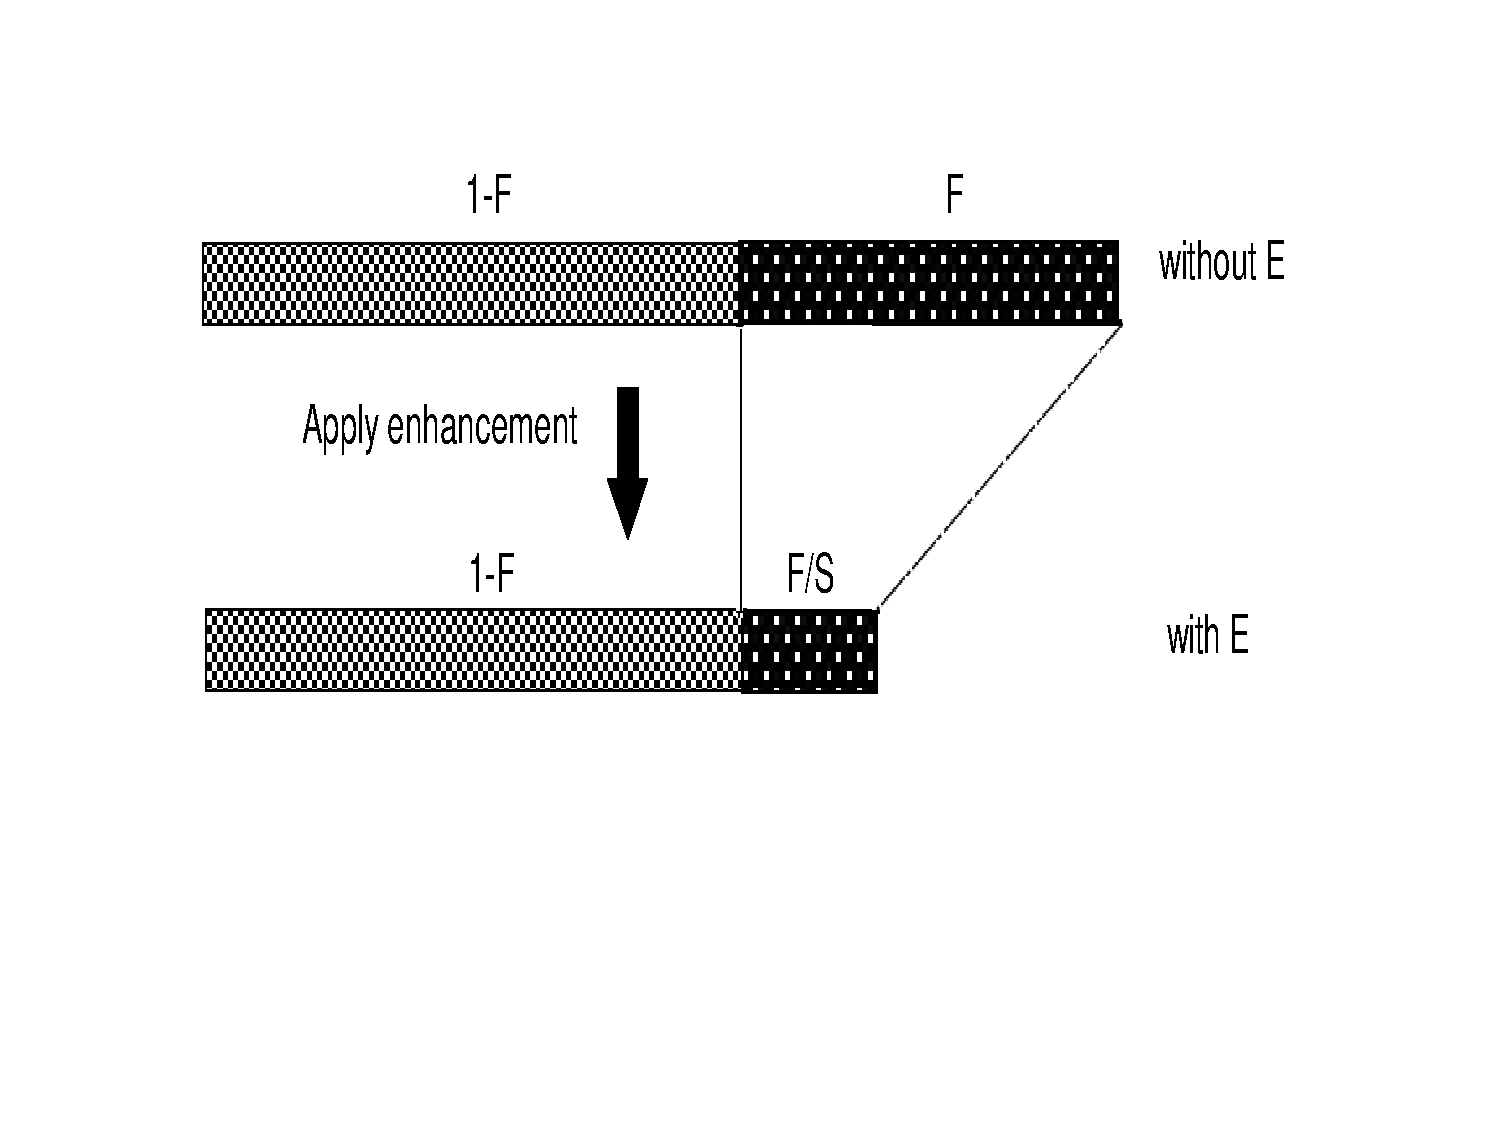
\includegraphics[width=50ex]{Figures/L2/Amdahl}\vspace{-15ex}
\caption{Enhancement $E$ accelerates a fraction $F$ of a program by a factor $S$.}
\label{fig:amdahl-assump}
\end{figure} 

Figure~\ref{fig:amdahl-assump} shows a scenario in which
an ``enhancement'' accelerates the computation of a fraction
$F$ of a program on a fixed dataset\footnote{
In general, a program running time is sensitive to the dataset,
so it does not makes sense to talk about speeding up a fraction
$F$ of a program in general---we need to fix the dataset.
} by a factor of $S$, while the other part of the program 
$1-F$ does not benefit from it.
(It is not important what the enhancement actually is,
or whether it is of software or hardware nature.)

In this scenario, the execution time of the enhanced program is:
\begin{center}
$T_{exe}(with E) = T_{exe}(without E)\times[(1-F) + \frac{F}{S}]$
\end{center}
Amdahl's Law correspond to (the interpretation of) three formulas:
one that computes the speedup of the enhanced program:
\begin{center}
$Speedup(E) = \frac{T_{exe}(without E)}{T_{exe}(with E)} = \frac{1}{(1-F)+\frac{F}{S}}$
\end{center}
and another two that compute an asymptotically-tight upper bound 
for the speedup when $S$ goes to infinity: 
\begin{center}
$Speedup(E) \leq \frac{1}{1-F}~~~~~$ and $~~~~~\lim_{S\to\infty}~Speedup(E) = \frac{1}{1-F}$
\end{center}

In essence, Amdahl's law shows that no matter how big the improvement is,
the overall application speedup is limited by the $1-F$ fraction that
does not benefit from the improvement.

\begin{figure}
\vspace{-4ex}
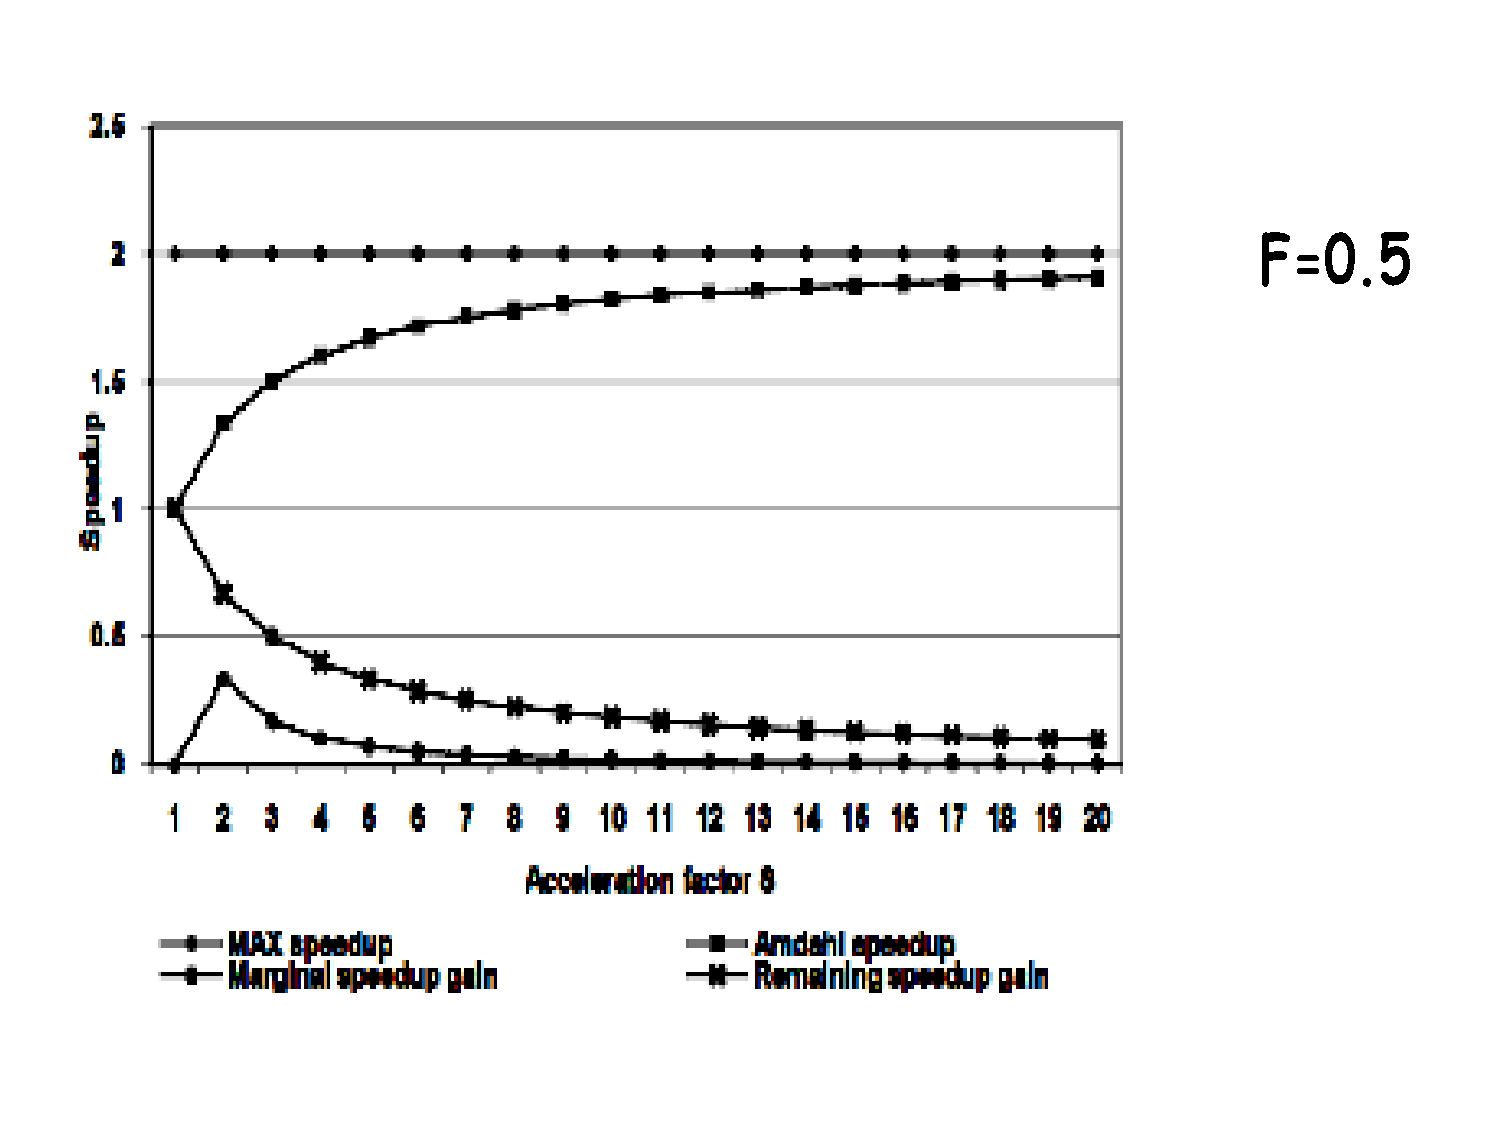
\includegraphics[width=90ex]{Figures/L2/AmdhalDimRet}\vspace{-7ex}
\caption{Interpretation of Amdahl's Law by Diminishing Returns. The $x$ and $y$ axis show the acceleration factor $S$ and the speedup, respectively. The lines appearing in the figure from top to bottom are: the maximal permitted speedup, the Amdahl's speedup, the remaining speedup gain, the marginal speedup gain (between two consecutive values of S).}
\label{fig:amdahl-interp}
\end{figure}

Figure~\ref{fig:amdahl-interp} shows a more detailed interpretation
of Amdahl's Law, specialized for the value $F = 0.5$, hence the maximal
speedup is $2\times$.   The figure demonstrates the law of diminishing
returns. It is reasonable to assume that every increment of $S$---shown
on the $x$ axis---requires the same amount of additional resources
(for enhancement). However, every increment of $S$ is less and less
rewarding globally. For example the step from $S=2$ to $S=3$ generates
an overall program speedup of $33\%$, while moving from $S=5$ to
$S=6$ generates a much smaller increase in speedup of only $6.67\%$. 
The moral of the story is to realize that some games cannot be 
won---the program speedup will never be higher than $2\times$---so
one should know when to stop, i.e., at the point when the next 
speedup gain will not justify the (extra) cost of the resources
necessary for implementing the next unit of enhancement.
In what hardware design is concerned, this would mean to implement
the ``common case\footnote{The common case is typically determined
by benchmarking.}'' in hardware (hence fast), and execute the rare
case in software (e.g., exceptions). 

\begin{figure}
\vspace{-4ex}
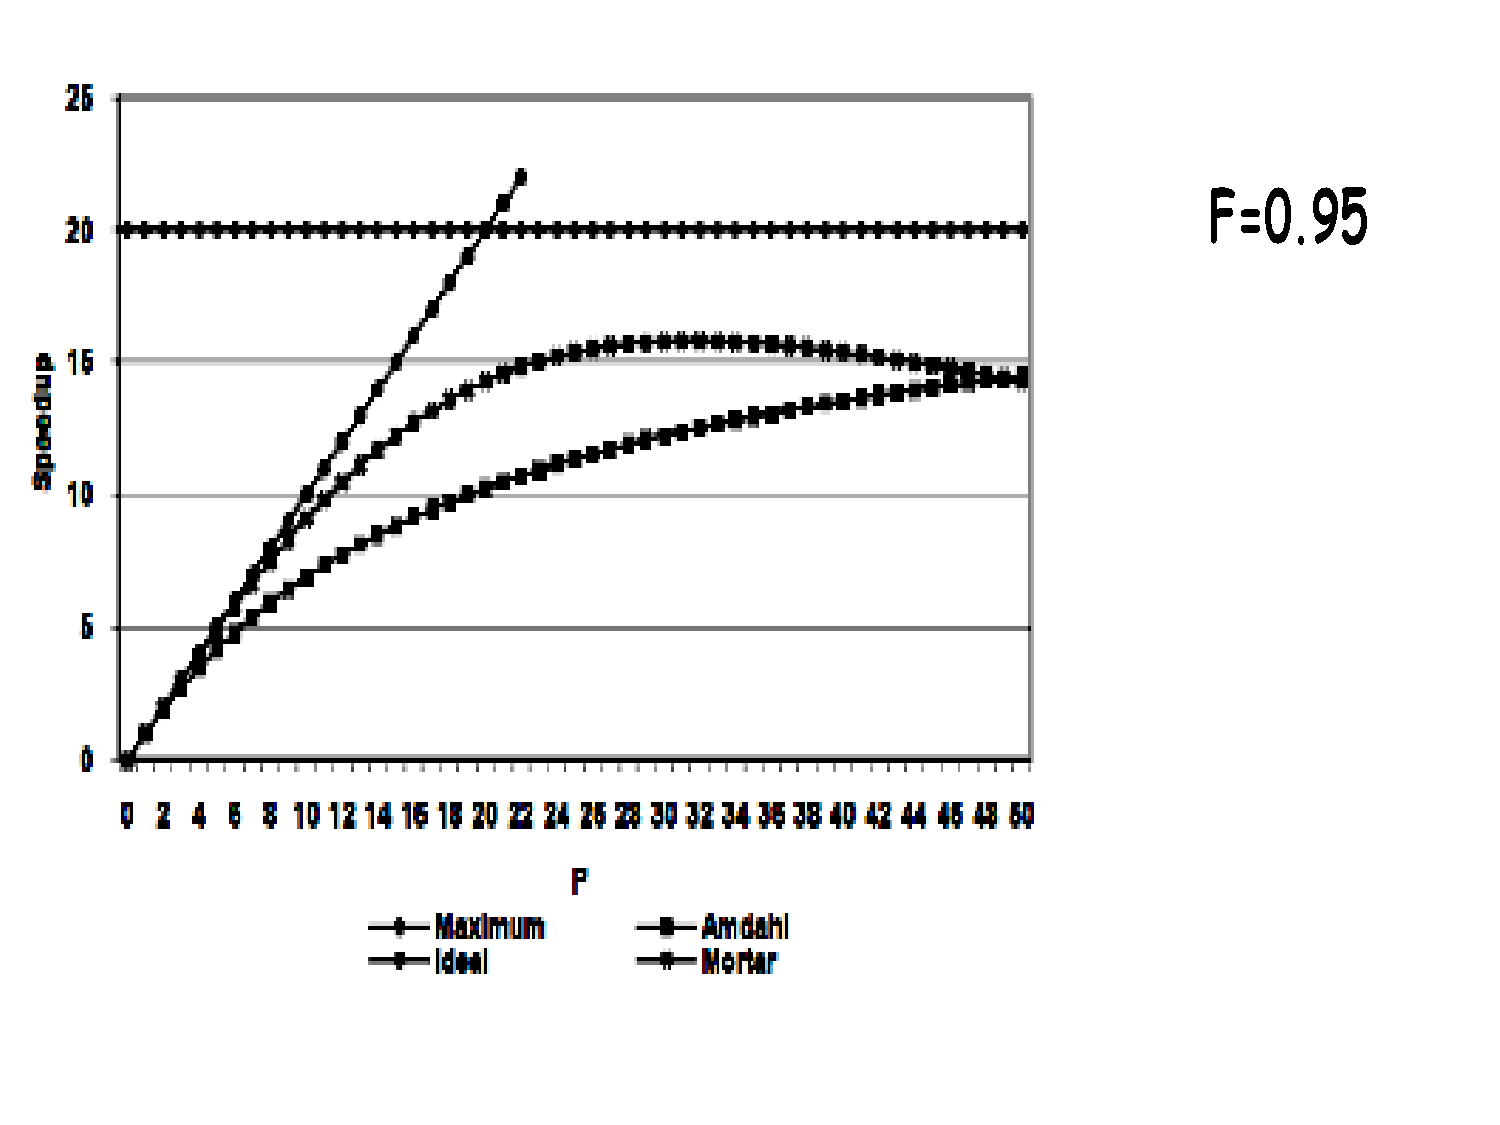
\includegraphics[width=90ex]{Figures/L2/AmdahlPar}\vspace{-7ex}
\caption{Demonstrating Amdahl's Law when the enhancement is 
parallel execution and $F=0.95$.\\ The mortar line shows a ``typical'' 
evolution of speedup in practice.}\vspace{-2ex}
\label{fig:amdahl-parallel}
\end{figure}

Figure~\ref{fig:amdahl-parallel} depicts the interpretation for
applying the Amdahl's law to the particular case of parallelism:
\begin{center}
$Speedup(P) = \frac{T_1}{T_P} = \frac{P}{F+P(1-F)}<\frac{1}{1-F}$
\end{center}
The specialization is straightforward: utilizing $P$ cores (rather 
than one) ideally results in a $P\times$ speedup. Actually, that 
is not quite true, since \emph{the occasional} super-linear speedup 
may be observed due to cache effects---the $P$ cores together have 
$P\times$ more cache than the uniprocessor, and applications 
with regular access patterns may benefit for the cache increase.
But typically, the speedup is sublinear even if $F=1$, because
for example threads might need to communicate and communication 
is expensive. One can observe that the Amdahl's law is unforgiving:
the figure uses $F=95$, which corresponds to $95\%$ of the runtime
being run in parallel; still the speedup is limited to $20\times$,
no matter how many cores you through at it.

The moral of the parallel case is different than the one for the
general hardware improvement. We do not advocate to bound/restrict 
the number of cores just because some applications are inherently
sequential and will not benefit for extra parallelism. Quite the
contrary: after all, we have seen that scaling hardware parallelism
is the only conceivably way (nowadays) of keeping the Moore's Law
alive. 

What we advocate is to never leave sequential any part of 
the program that can possibly be parallelized. \emph{In other words, 
when developing parallel code, we must reason as if the hardware 
has an unlimited/infinity number of cores.}

Let me stress this further with an example that may catch your attention: 
assume the student has parallelized $99.9\%$ percent of the runtime of 
the application subject to the group project/exam. The student may feel 
entitled to receive the maximal grade, but the teacher might argue 
otherwise. The reason is that the GPUs that you are using in the PMPH 
course currently support $2880$ cores each.   Assume for the sake of 
the argument that each core run as fast as the CPU (they do not!). 
Applying Amdahl's law for $F=99.9\%$ results in a limiting
$1000\times$ speedup. This means that the student is only utilizing
about one third of the compute power provided by one GPU, and $35\%$
is a \emph{\bf failing grade}!


\subsubsection{Work-Depth Asymptotic Behavior of a Parallel Program}
\label{subsubsub:work-depth}
$\mbox{ }$\\

While there is a trend towards simplifying hardware, current hardware
remains way too complex for developing cost models based on them.
At least in what teaching is concerned, using a realistic hardware
model will put us in danger of ``missing the forest for the trees''. 
We will discuss parallel-program properties by reasoning about the
program execution on a very simple and idealized hardware model, 
named the parallel random access machine (PRAM). PRAM focuses on
(data) parallelism and completely ignores issues related to 
synchronization and communication. It assumes that:
\begin{itemize}
    \item there are $P$ processors that are connected to shared memory,

    \item each processor has an unique identifier/index $0 \leq i < P$,

    \item the execution happens in single-instruction multiple data (SIMD)
            fashion, which means that all cores execute in lock step---i.e.,
            a core cannot start the next instructions until all cores have
            completed executing the current instruction. Please note that
            in the case of an \lstinline{if-then-else}, the processors that
            did not take the \lstinline{then} branch must wait until all the
            other processors has finished executing the \lstinline{then} branch,
            before starting to execute the \lstinline{else} branch, and
            similar for the \lstinline{else} branch.

    \item each parallel instruction takes unit time (the same amount of time
            no matter whether it is a simple or complex arithmetic operation
            or a memory access).

    \item each processor has a flag that controls whether it is active in the
            execution of an instruction (for example in order to implement
            \lstinline{if-then-else}). If the processor is not active, then
            its {\tt noop} does not count towards the work complexity
            (but it counts towards the depth complexity, because it is
            part of a SIMD computational step).
\end{itemize}

We are ready to define the work-depth asymptotic behavior of a parallel
program on a PRAM machine. The work and depth computation assumes an
infinity number of processors ($P = \infty$).
\begin{itemize}
    \item \emph{\bf The work complexity} is the total number of operations
        performed to execute the program, i.e., the sum across all processors.
        We denote work by $W(n)$, where $n$ is related to the size of the
        dataset/workload.
    
    \item \emph{\bf The depth or step complexity}, denoted by $D(n)$ is 
        the number of sequential steps needed to execute the program.

    \item \emph{\bf A parallel implementation is work efficient} if its work
        complexity is asymptotically equal to that of the best sequential 
        implementation of the same algorithm.
\end{itemize} 

If we know (have computed) the work and depth of an implementation, then 
Brent's theorem specifies ``good'' complexity bounds for a PRAM that has
a finite number of $P$ cores, where by good we mean tight enough to be 
useful (for reasoning) in practice.

\begin{mytheo}[Brent's Theorem]\label{Brent-TH}
$\mbox{ }$\\
A parallel implementation that has depth $D(n)$ and work $W(n)$
can be simulated on a $P$-processor PRAM in time complexity $T$ 
such that:
\begin{center}
$\frac{W(n)}{P} \leq T \leq \frac{W(n)}{P} + D(n)$
\end{center}
\end{mytheo}

\subsubsection{Demonstrating Work-Depth Computation for Reduction}
\label{subsubsub:work-depth}
$\mbox{ }$\\

\begin{figure}
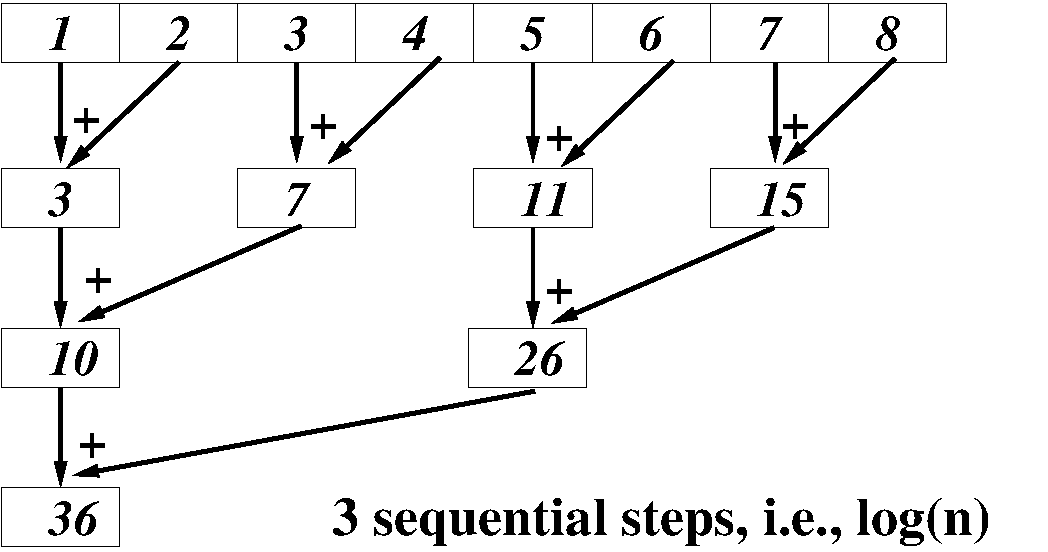
\includegraphics[width=40ex]{Figures/L1/ReduceEg.pdf}
\caption{Parallel execution of \lstinline{reduce} requires
        a sequence of \lstinline{log(n)} parallel operations
        ({\tt n} is the array length).}
\label{fig:red-tree-again}
\end{figure} 


The reduction tree for summing up (\lstinline{reduce (+) 0}) the elements 
of an array of $8$ elements is shown (again) in \cref{fig:red-tree-again}.
It is intuitively easy to generalize the work and depth for an array of
$n$ elements, which is summed up using $\frac{n}{2}$ processors:
\begin{itemize}
    \item the work is $W(n) = n$, hence parallel summation is work efficient
        because the best sequential algorithm still performs $O(n)$ steps;
    \item the depth is $D(n) = log(n)$, i.e., number of sequential steps;
    \item the optimized runtime on $P$ processors is actually 
            \emph{$O((n/P) + log(P))$.} This can be achieved by
            transforming the program according to \cref{Lemma-Map-Red}. 
            We recall that the ``Optimized-Map-Reduce Lemma'' says that
            a \lstinline{map-reduce} composition can be executed by:
        \begin{itemize}
            \item[(1)] chunking the input array into $P$ subarrays of roughly-equal 
            sizes,
            \item[(2)] then processing each subarray \emph{sequentially} on a 
            different processor, but \emph{in parallel} across subarrays,
            \item[(3)] the reducing the results of the $P$ subarrays
            in parallel by means of a reduction tree.
        \end{itemize}
            Step (1) and step (2) are fully parallel and take $O(n/P)$ time, 
            while step (3) requires 
            a reduction tree on $P$ elements, which takes $O(lg \ P)$ time (depth).
    \item one can now verify that Brent's lemma:\\
            \begin{center} $O(\frac{n}{P}) ~\leq ~O(\frac{n}{P} + log(P)) ~\leq~ O(\frac{n}{P} + log(n))$ \end{center}
          gives bounds which are good approximations (for the assumed $P \leq \frac{n}{2}$) 
            and allows us to reason on the essence rather than overthink the 
            impact of optimizations.
\end{itemize}

\begin{figure}
\begin{lstlisting}[mathescape=true]
Input:  array A of n=2$^k$ elems of type T
        $\oplus : T \rightarrow T \rightarrow T$ associative
Output: S = $\oplus_{j=1}^{n} a_j$

1.  forall i = 0 to n-1 do
2.    B[i] $\leftarrow$ A[i]
3.  endfor

4.  for h = 1 to k do
5.    forall i = 0 to n-1 by 2$^h$ do 
6.      B[i] $\leftarrow$ B[i] $\oplus$ B[i+2$^{h-1}$]
7.    endfor
8.  endfor
9.  S $\leftarrow$ B[0]  
\end{lstlisting}\vspace{-4ex}
\caption{Imperative, low-level pseudocode for parallel array summation.}
\label{fig-red-imp-pseudo}
\end{figure}

We have so far derived the work-depth complexity of array summations
in an intuitive way, by abstracting out the information depicted in 
a picture.   The question is: ``Can we also do this in a systematical
way for an arbitrary code?'' It turns out the answer is positive,
as demonstrated by the following analysis of the low-level (imperative)
pseudocode presented in \cref{fig-red-imp-pseudo}. The analysis
proceeds bottom-up, by which we mean that we go in-order across
constructs at the same level and innermost-to-outermost in
nests:

\begin{itemize}
    \item The parallel loop between lines $1-3$ has 
            $D_{1-3}(n) = \Theta(1)$, and $W_{1-3}(n) = \Theta(n)$,
    \item The parallel loop between lines $5-7$ has
            $D_{5-7}(n) = \Theta(1)$, and $W_{5-7}(n,h) = \Theta(n/2^h)$,
    \item The sequential loop between lines $4-8$ executes $k$ 
            iterations ($n = 2^k$, hence $k = lg \ n$), each 
            consisting of the parallel loop $5-7$, 
            hence it has:
        \begin{itemize}
           \item depth $D_{4-8}(n) = k \times D_{5-7}(n) = \Theta(lg \ n)$, and
           \item work $W_{4-8}(n) = \sum_{h=1}^k W_{5-7}(n,h) = \Theta(\sum_{h=1}^k (\frac{n}{2^h}) ) = \Theta(2 n (1 - \frac{1}{2^{k+1}}) ) = \Theta(2 n (1 - \frac{1}{2 n}) ) = \Theta(n)$
        \end{itemize}
    \item The statement on line $9$ trivially has $D_{9}(n) = \Theta(1)$, $W_{9}(n) = \Theta(1)$,\bigskip
    \item Thus the depth and work for the entire program are
        \emph{$D(n) = \Theta(lg \ n), ~~\mbox{\tt and}~~ W(n) = \Theta(n)$}, respectively!
    \item By Brent's Theorem, it follows that the actual runtime is bounded by:
            $\frac{n}{P} \leq Runtime \leq \frac{n}{P} + lg \ n$
\end{itemize}

\subsubsection{Naive and Native Implementation of Reduction in Futhark}
\label{subsubsub:work-depth}
$\mbox{ }$\\

The previous section has shown that a reduction can be easily
implemented based on \lstinline{map}s and sequential loops.
It is natural to ask then, why does reduction need to be a
first-class citizen of a data-parallel language, when it can
be easily be provided as part of a library? 

We first provide an intuitive demonstration by implementing
reduction in the Futhark data-parallel language and comparing
the performance of our program with the natively supported
reduction. This also allows us to get acquainted with Futhark,
which will be used in PMPH exercises and so on.

\begin{figure}
\begin{lstlisting}[mathescape=true]
-- Reduction by hand in Futhark implemented in file: red-by-hand.fut
-- ==
-- compiled input {
--    [1.0f32, -2.0, -2.0, 0.0, 0.0, 0.0, 0.0, 0.0, 
--     3.0, 4.0, -6.0, 1.0, 2.0, -3.0, 7.0, 2.0]
-- }
-- output {
--    7.0f32
-- }
-- compiled input @ data/f32-arr-16777216.in
-- output { 3091.746094f32 }

-- For simplicity, assumes that n is 2^k
let main [n] (a : [n]f32) : f32 =
  let k = t32 <| f32.log2 <| r32 n
  let b = 
    loop b = a for h < k do
        let n' = n >> (h+1)
        in  map (\i -> unsafe (b[2*i]+b[2*i+1]) ) (iota n')
  in b[0]
\end{lstlisting}\vspace{-4ex}
\caption{Futhark Implementation for Summing Up an Array of Single-Precision Floats}
\label{fig:futhark-red}
\end{figure}

The Futhark implementation of the reduction pseudocode discussed
in the previous section is presented in \cref{fig:futhark-red}.
In the following, we will explain the code:
\begin{itemize}
    \item[(1)] In Futhark comments start with token {\tt --} and expand
            until the end of the line. However, an uninterrupted 
            sequence of comment lines that start a source file 
            (after the \lstinline{-- ==} comment) define 
            reference input-output datasets for automatic testing
            or benchmarking:

        \begin{itemize}
            \item The first dataset is directly specified:
            the input consists of an array of $16$ single-precision
            floats (\lstinline{f32}), using the common array literal 
            notation {\tt [a$_1$, $\ldots$, a$_n$]}, and the reference
            result is a single precision float {\tt 7.0f32}.

            \item The second dataset is held in a file 
            (\lstinline{-- compiled input @ data/f32-arr-16777216.in}),
            that stores an array of length $16777216$, but the result
            is given explicitly, albeit it can similarly be stored in
            a file (e.g., \lstinline{-- output @ data/f32-arr-16777216.out}).

            \item Assuming the name of the file is {\tt red-by-hand.fut},
                  compilation for GPU can be carried out with the command
            {\tt \$ futhark-opencl red-by-hand.fut} and compilation for
                  sequential C can be performed with  
            {\tt \$ futhark-c red-by-hand.fut}; both will result in an executable
            named {\tt red-by-hand}, which can be run on a dataset with the
            command:\\ 
            {\tt \$ red-by-hand -t /dev/stderr -r 10 < data/f32-arr-16777216.in}\\
            The {\tt -t} option records the program runtime (in microseconds)
            in the next-specified file; in our case this is displayed 
            in {\tt /dev/stderr}. The reported runtime {\bf does not include}:
            \begin{itemize} 
               \item the CPU-to-GPU transfer of the program input and the
            GPU-to-CPU transfer of the program result. 
               \item the OpenCL context creation and OpenCL kernel compilation.
            \end{itemize}
            Option {\tt -r 10} specifies that the runtime should be averaged
                across $10$ runs.
            If one wishes to inspect various profiling information, the
            program can be run with option {\tt -D}; this is especially
            useful when program compilation generates a number of kernels.

            \item Testing and benchmarking across the datasets specified in
            the source file itself can be carried out with the commands:\\
             {\tt \$ futhark-test  --compiler=futhark-opencl red-by-hand.fut}, or\\
             {\tt \$ futhark-bench --compiler=futhark-opencl red-by-hand.fut}

            \item random (uniformly-distributed) datasets can be created with
            the {\tt futhark-dataset} command (see help with the {\tt --help} option).
            An dataset consisting of an array of $16777216$ \lstinline{f32}
            elements can be produced and saved in file  {\tt data/f32-arr-16777216.in}
            by using the command:\\
            {\tt futhark-dataset -b --f32-bounds=-1.0:1.0 -g [16777216]f32 > data/f32-arr-16777216.in}
            
        \end{itemize}

    \item[(2)] Program execution starts with function {\tt main}.
          A function declaration starts with keyword \lstinline{let}
            followed by the function's name, which is optionally
            followed by declaring a set of variables that will be used
            to denote array sizes, for example \lstinline{[n][m][p]},
            followed by a sequence of typed formal arguments,
            and by the return type of the function.
        \begin{itemize}
          \item Our \lstinline{main} has one formal parameter, denoted
            {\tt a} which is an unidimensional array of single-precision 
            floats of length {\tt n}, i.e., (\lstinline{a: [n]f32}).   
          \item A three-dimensional array
            in which the sizes of the first and last dimension are {\tt n}
            and the size of the second dimension is {\tt m} would
            be written as \lstinline{[n][m][n]f32}, and {\tt m} would
            need to be declared similar to {\tt n}, i.e., {\tt [n][m]}.   
          \item In our case the result is a scalar: {\tt f32}.
                The programmer has to be a bit careful with the
                sizes of an array result type: a size which is declared
                in the optional part can be used in the array-result
                type if and only if it has been used in one of the
                formal array arguments. For example,
                \lstinline{let main [n] (a : [n]f32) : [n]f32 = ...}
                is legal and says that the input and result array should
                have the same length, but 
                \lstinline{let main [n] (m : f32) : [n]f32 = ...} is
                illegal because {\tt n} cannot be deduced from the inputs.
                In the latter case, what the user intends is probably 
                \lstinline{let main (n : i32) (m : i32) : [n]f32 = ...}.
        \end{itemize}
    \item[(3)] The program input and result  
            must be specified in tuple of arrays form (or structure of arrays AoS).
            (Note that this restriction only refers to the {\tt main} function   
            and entry points; all other code may use array-of-tuple form.)
            This is because the Futhark compiler automatically performs
            the AoS-to-SoA transformation in early compilation stages,
            but it obviously cannot also transform the program input.
            For example, it would be illegal to pass {\tt main}
            a formal argument \lstinline{b : [n](f32,f32)} or \lstinline{c : (f32, f32)}; 
            these should be split into two arguments each: 
            \lstinline{(b1: [n]f32) (b2: [n]f32)} or \lstinline{(c1: f32) (c2: f32)}.

    \item[(4)] The body of the {\tt main} is a \lstinline{let} expression.
        \begin{itemize}
              \item[1.] {\tt k} is bound to the value of {\tt log2 n}:\\
                \lstinline{let k = t32 <| f32 . log2 <| r32 n}\\
                where {\tt n} is assumed to be a power of two, and {\tt <|} pipes
                the right-hand side result to the left-hand side function (call): 
                \begin{itemize} 
                \item \lstinline{r32 n} transforms the $32$-bit integer \lstinline{n : i32}
                to a single precision float (\lstinline{f32}).
                \item \lstinline{f32.log2} calls the base-$2$ logarithm of the
                \lstinline{f32} module.
                \item \lstinline{t32} truncates the float argument to an \lstinline{i32}.
                \end{itemize}
              \item[2.] {\tt b} is defined to be the result of the \lstinline{loop}
                expression: \lstinline{loop b = a for h < k do body}, which is always
                executed sequentially: 
                \begin{itemize} 
                    \item {\tt b} is a variable bounded in the loop context, whose 
                value is variant across different iterations of the loop: it is initialized 
                upon loop entry with the value of {\tt a}, and the result of
                the loop {\tt body} will give the value of {\tt b} to be used by
                the next iteration of the loop.
                    \item the loop runs {\tt k} iterations (we recall that {\tt n = $2^k$})
                and {\tt h} takes values in {\tt 0, $\ldots$, k-1} in different iterations.
                Loops may also iterate across elements of an array using the more direct
                notation \lstinline{for x in xs}, such that {\tt x = xs[i]} in some iteration 
                {\tt i}.
                \end{itemize}
            \item[3.] The body of the loop consists of a \lstinline{let} expression:
            \begin{itemize}
                \item \lstinline{let n ' = n >> (h+1)} which binds {\tt n'} to the
                    value obtained by bit-shifting {\tt n} in the right direction with
                    {\tt h+1} bits, i.e., $n' = \frac{n}{2^{h+1}}$.
                \item and results in the application of \lstinline{map}
                    second-order array combinator (SOAC):\\
                    \lstinline{map (\i -> unsafe (b[2*i]+b[2*i+1]) ) (iota n')}
                    \begin{itemize}
                        \item the array input of the \lstinline{map} is \lstinline{iota n'}
                        which corresponds to the array {\tt [0,1,$\ldots$,n'-1]}.
                        \item the mapped anonymous (lambda) function is 
                        \lstinline{\i -> unsafe (b[2*i]+b[2*i+1]}.
                    \end{itemize}
                    Please note that the Futhark implementation differs from the
                    imperative-pseudocode shown in \cref{fig-red-imp-pseudo} in that
                    each iteration of the Futhark look computes an array result
                    of half the size of the input {\tt b}: iterations {\tt h=0},
                    {\tt h=1} and {\tt h=k-1} result in arrays of length 
                    $n' = \frac{n}{2^1}$, $n' = \frac{n}{2^2}$ and $n' = \frac{n}{2^k}=\frac{n}{n}=1$,
                    respectively.  That is the reason why all iterations use \lstinline{map}
                    with the same function \lstinline{\i -> unsafe (b[2*i]+b[2*i+1]}.
            \end{itemize}
            \item[4.] Finally the loop execution results in an array {\tt b} 
                containing one element, and the {\tt main} function returns
                the (first) element of {\tt b} (i.e., {\tt b[0]}).
        \end{itemize}

\end{itemize}

The second program, named {\tt red-native.fut} simply consists
of the code\\ 
\lstinline{let main [n] (a : [n]f32) : f32 = reduce (+) 0 a}
and we add the header used for testing/benchmarking.

Compiling and running the two programs on {\tt gpu04-diku-apl} 
shows that the native reduce is about a factor $8\times$ faster 
than our by-hand implementation ({\tt red-by-hand.fut}) based on
iterative \lstinline{map}s, on dataset {\tt data/f32-arr-16777216.in}:
 $321 \mbox{\tt vs} 2511$ microseconds.

The reason is that the code-generation of the native construct
benefits from an optimized code generation that executes \emph{one}
kernel\footnote{
The code generation of {\tt reduce} actually runs two kernels,
but the second one takes negligible time}
that performs about $n$ reads from global memory and much fewer 
writes to global memory, while using internally scratchpad (fast) 
GPU memory. 

In contrasts the discussed implementation ({\tt red-by-hand.fut})
executes a $24$-iteration loop ({\tt h = 0,$\ldots$,23}), in which 
each loop iteration calls a kernel corresponding to the \lstinline{map}
of size $n' = \frac{n}{2^{h+1}}$. The \lstinline{map} reads $2n'$ and 
writes $n'$ elements from/to global memory.
In total this implementation performs about $4 n$ reads and $2 n$ writes
from/to global memory.  The remaining difference can be explained 
by the overhead required to call an OpenCL kernel.

This is one of the reasons for which it makes sense to have second-order
array combinators (SOACs) such as \lstinline{reduce} and \lstinline{scan} as
first-class citizens in the data-parallel language. The other reason
corresponds to the algebraic properties of such operators: for example
the composition of a reduce and a map can be fused in a more
advanced construct~\cite{Futhark:redomap,Futhark:segredomap}, by a rule
similar to \cref{Lemma-Map-Red} which, similarly requires to read the 
input array once from global memory. 
Such high-level fusion rules would not be possible if we would implement
the {\tt reduce} in the library based on iterative applications of \lstinline{map};
it is even difficult to see how fusion could be applied in such a context.

\subsection{Other Parallel Operators, Examples of Nested-Parallel Applications}
\label{subsec:nest-par-app}

This section is organized as follows: 
\begin{itemize}
    \item \cref{subsubsub:var-par-ops} introduces
the type and semantics of several parallel operators commonly used in 
(functional) data-parallel languages. 
    \item \cref{subsubsub:scan-impl} presents
a possible, work-efficient implementation of the \lstinline{scan} 
(a.k.a. parallel-prefix sum) operator, which is a basic-block of
parallel programming, and shows how a segmented scan operator can
be easily written in terms of \lstinline{scan}. 

    \item \cref{subsubsub:filter-impl} shows a possible implementation of
\lstinline{filter} based on \lstinline{map} and \lstinline{scan}
and \lstinline{scatter} (parallel write) operators.

    \item The remaining (sub)sections demonstrate how 
        several applications can be constructed as puzzles from a nested
        composition of such operators:
        \begin{itemize}
        \item \cref{subsubsub:sparse-mat-vec-mult} briefly discusses
            the multiplication of a sparse matrix with a dense vector,
            and in particular introduces the notion of 
            \emph{\bf data flattening}.
        \item \cref{subsubsub:primes} presents three implementations for
            computing all prime numbers less then a certain input: 
            the first version provides the intuition, but does not have 
            the optimal depth; the second version fixes depth optimality,
            but this does not means it is necessarily best in practice;
            the last version is work inefficient but has a structure
            that makes it efficient for GPU hardware.
        \item Finally, \cref{subsubsub:quicksort} looks at the implementation
            of quicksort.
        \end{itemize}
\end{itemize}


\subsubsection{Types and Semantics of Various Parallel Operators}
\label{subsubsub:var-par-ops}
$\mbox{ }$\\

We start the discussion with \lstinline{zip} and \lstinline{unzip} operators:
\lstinline{zip} receives two arrays of the same length {\tt n} and produces
an array of tuples of length {\tt n} by pairing-up the elements at the same
index of the two arrays. \lstinline{unzip} is the inverse of \lstinline{zip}, 
i.e., \lstinline{unzip=zip}$^{-1}$:
\begin{lstlisting}[mathescape=true]
zip : $\Pi$n. [n]$\alpha_1$ $\to$ [n]$\alpha_2$ $\to$ [n]($\alpha_1,\alpha_2$)
zip [a$_1$,$\ldots$, a$_n$] [b$_1$,$\ldots$, b$_n$] = [(a$_1$,b$_1$),$\ldots$,(a$_n$,b$_n$)]
\end{lstlisting}\vspace{-1ex}

\begin{lstlisting}[mathescape=true]
unzip : $\Pi$n. [n]($\alpha_1,\alpha_2$) $\to$ ([n]$\alpha_1$, [n]$\alpha_2$)
unzip [(a$_1$,b$_1$),$\ldots$,(a$_n$,b$_n$)] = [a$_1$,$\ldots$, a$_n$] [b$_1$,$\ldots$, b$_n$]
\end{lstlisting}\vspace{-2ex}

Please note that our semantics differs from the one in Haskell, which would allow
two list of different length and would result in an array of tuples whose length
is the minimum of the input-array lengths.  In Futhark \lstinline{zip/unzip} are
syntactic sugar: they are supported in the source language, but are eliminated
(compiled away) in an early compiler stage that systematically rewrites the 
program to a tuple-of-arrays form.

We use the following array constructors:  
\begin{lstlisting}[mathescape=true]
iota : (n: i32) $\to$ [n]i32
iota n = [0,$\ldots$, n-1]
\end{lstlisting}\vspace{-1ex}

\begin{lstlisting}[mathescape=true]
replicate : (n: i32) $\to$ $\alpha$ $\to$ [n]$\alpha$
replicate n a = [a,$\ldots$, a]
\end{lstlisting}\vspace{-2ex}
\lstinline{iota n} creates an arrays of integral elements starting from {\tt 0} 
to {\tt n-1}, and \lstinline{replicate n a} creates an array of length {\tt n} 
filled with the same element {\tt a}. \lstinline{iota} can be used to create
the iteration space, for example in the case when the parallel operator needs
to access several elements of the input array in each iteration; we have seen
such an example in the case of the naive-reduce implementation:
\lstinline{map (\i -> unsafe (b[2*i]+b[2*i+1]) ) (iota n')}.
\lstinline{replicate} is typically used for initializing an array which will
be subject to a scan or to in-place updates.   

\begin{figure}
\begin{lstlisting}[mathescape=true]
map  : ($\alpha\to\beta$) $\to$ $\Pi$n. [n]$\alpha$ $\to$ [n]$\beta$
map  f [a$_1$, $\ldots$, a$_n$] = [f a$_1$, $\ldots$, f a$_n$]
map2 : ($\alpha1\to\alpha_2\to\beta$) $\to$ $\Pi$n. [n]$\alpha_1$ $\to$ [n]$\alpha_2$ $\to$ [n]$\beta$
map2 f [a$_1$, $\ldots$, a$_n$] [b$_1$, $\ldots$, b$_n$] = [f a$_1$ b$_1$, $\ldots$, f a$_n$ b$_2$]
map3 : $\ldots$

reduce : ($\alpha \to \alpha \to \alpha$) $\to$ $\alpha$ $\to$  $\Pi$n. [n]$\alpha$ $\to$ $\alpha$
reduce $\oplus$ 0$_{\oplus}$  [a$_1$, $\ldots$, a$_n$] = 0$_{\oplus}$ $\oplus$ a$_1$ $\oplus$ $\ldots$ $\oplus$ a$_n$

scan : ($\alpha \to \alpha \to \alpha$) $\to$ $\alpha$ $\to$ $\Pi$n. [n]$\alpha$ $\to$ [n]$\alpha$
scan $\oplus$ 0$_{\oplus}$ [a$_1$, $\ldots$, a$_n$] = [0$_{\oplus}$ $\oplus$ a$_1$, $\ldots$, 0$_{\oplus}$ $\oplus$ $\ldots$ $\oplus$ a$_n$]

filter : ($\alpha$ $\to$ Bool) $\to$ $\Pi$n. [n]$\alpha$ $\to$ [m]$\alpha$   (where m $\leq$ n)
filter p [a$_1$, $\ldots$, a$_n$] = [a$_{k_1}$,$\ldots$, a$_{k_m}$]
  such that k$_1$ < k$_2$ < $\ldots$ < k$_m$, and denoting by $\overline{\mbox{\tt k}}$ = {k$_1$,$\ldots$, k$_m$},
  we have (p a$_j$ == true) $\forall$ j $\in$ $\overline{\mbox{\tt k}}$, and (p a$_j$ == false) $\forall$ j $\not\in$ $\overline{\mbox{\tt k}}$
\end{lstlisting}\vspace{-4ex}
\caption{Types and Semantics of \lstinline{map}s, \lstinline{reduce}, \lstinline{scan}, \lstinline{filter}.}
\label{fig:futhark-par-ops}
\end{figure}

Figure~\ref{fig:futhark-par-ops} shows the types and semantics of several second-order
array combinators (SOACs). We have already introduce \lstinline{map} and 
\lstinline{reduce} combinators. For ease of notation we will also introduce
\lstinline{map2} which receives as arguments a binary function {\tt f} and 
two input arrays of the same length, and produces an array by applying {\tt f}
to corresponding elements from the first and second arrays, respectively. 
Similar definitions are possible for {\tt map3} and so on.

\lstinline{scan} is commonly known as parallel-prefix sum, since it produces
an array of the same length as the input by starting with the first element,
then applying the operator between the first two elements, then applying the
operator between the first three elements, and so on, until the last element
corresponds to the result of reducing the array. Please note that, similar to
\lstinline{reduce}, \lstinline{scan}'s binary operator $\odot$ must be associative
and {\tt e$_\odot$} must be its neutral element! Please also note that
the provided version of \lstinline{scan} is \emph{inclusive}; an \emph{exclusive}
\lstinline{scan} would produce an array starting with the neutral element and
ending with the reduction of the first {\tt n-1} elements. The work and depth
of \lstinline{scan} is also similar to \lstinline{reduce}: $O(n)$ and $O(lg~n)$,
respectively.

Finally, \lstinline{filter} receives as argument a predicate {\tt p} 
(i.e., a function of type $\alpha\to${\tt{}Bool}) and an input array,
and it filters-out from the input array all the elements that do not
succeed under the predicate (i.e., indexes {\tt j} such that 
{\tt p a$_j$ = }\lstinline{false}). Please note that (i) the result
elements respect the relative order in which they appear in the input
array, and that (ii) the size of the result array is necessarily 
less than or equal to that of the input array. The work and depth
of \lstinline{filter} is similar to \lstinline{scan} 
($O(n)$ and $O(lg~n)$), because its implementation uses \lstinline{scan}. 

We conclude this subsection by introducing \lstinline{scatter},
a very important operator used for updating in parallel some of 
the indices of an arrays, where the updated indices do not necessarily
follow any regular pattern, i.e., think parallel random writes.
Its type is:\\
\lstinline{scatter}{\tt : $\Pi$ n. *[n]$\alpha~\to~\Pi$ m. [m]}\lstinline{i32}
{\tt$\to$ [m]$\alpha$ $\to$ [n]$\alpha$}\\
which means that it receives as arguments a base array of length {\tt n},
and two arrays of length {\tt m} holding the to-be-updated
indices and corresponding values, respectively, and produces an array
of size {\tt n} by applying the updates. We make the following
important observations:
\begin{itemize}
    \item[(1)] The star {\tt *} in front of the type of the first input 
        array specifies that the array is going to be consumed---since
        the update is performed in place, it means that any following 
        reference to that array is \emph{illegal}! 
    \item[(2)] Furthermore, the first input array cannot alias the other two 
        array arguments. This would not be necessary on a PRAM machine
        with an infinity number of cores that execute in SIMD fashion,
        but such hardware does not exist in practice.
    \item[(3)] The depth of \lstinline{scatter} is $O(1)$, and its work is 
        $O(m)$---meaning, it does not depend on {\tt n}, the size of 
        the to-be-updated array.
\end{itemize}
For programming convenience (e.g., padding), we enrich the semantics
of \lstinline{scatter} by requiring that the indices that are 
outside the bounds of the input array are simply ignored (are not
updated). As such {\tt n} and {\tt m} are in no relation with
each other: it can be that {\tt n<m} or {\tt n==m} or {\tt n>m}. 

We conclude with an example that hopefully clarifies how 
\lstinline{scatter} works:
\begin{lstlisting}[mathescape=true]
X (input  array) = [a$_0$, a$_1$, a$_2$, a$_3$, a$_4$, a$_5$]
I (index vector) = [2, 4, -1, 1]
D (data  vector) = [b$_0$, b$_1$, b$_2$, b$_3$]
scatter X I D    = [a$_0$, b$_3$, b$_0$, a$_3$, b$_1$, a$_5$]
\end{lstlisting}\vspace{-2ex}


\subsubsection{Implementation of Scan and Segmented Scan}
\label{subsubsub:scan-impl}
$\mbox{ }$\\

We start by emphasizing again that, similar to \lstinline{reduce},
\lstinline{scan} requires an \emph{\bf associative} binary operator,
and the neutral element of the monoid induced by that operator.

\begin{figure}
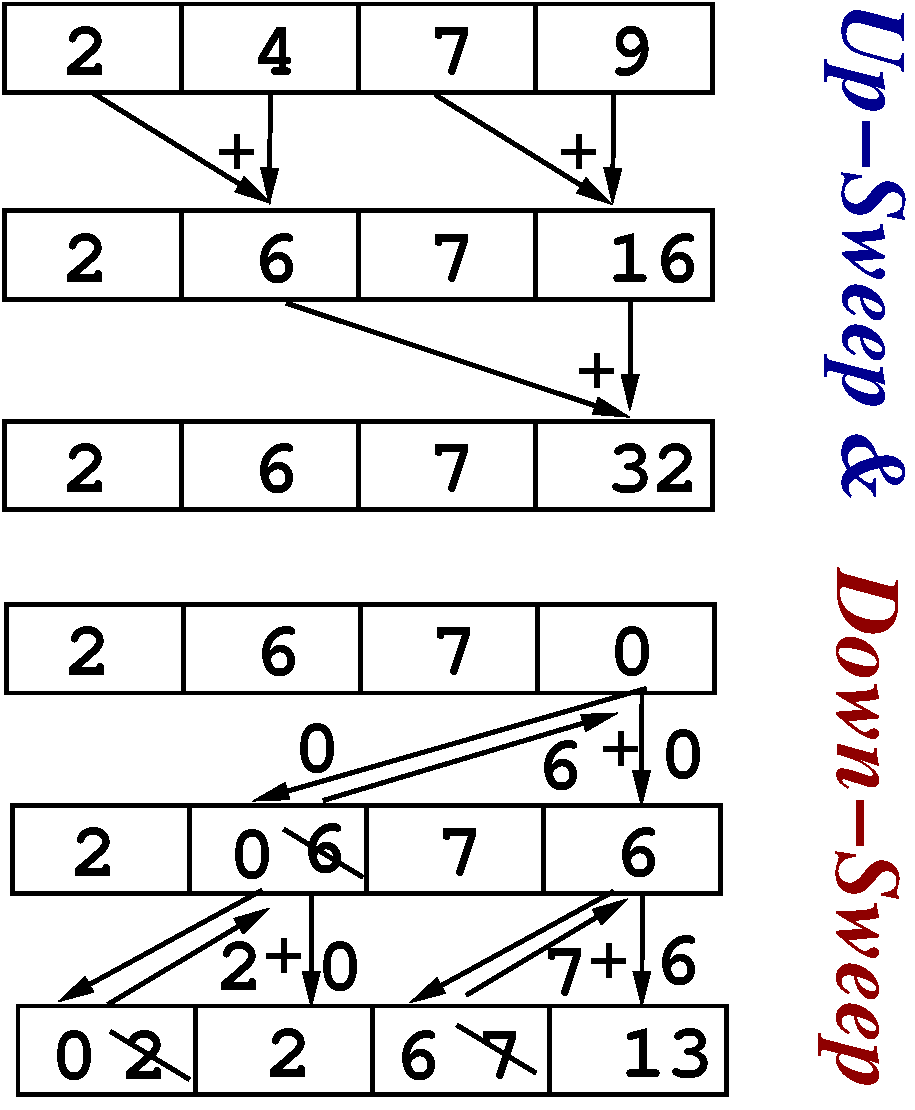
\includegraphics[height=33ex]{Figures/L2/ScanEg.pdf} 
\caption{Parallel execution of \lstinline{scan} for a $4$-element array.}
\label{fig:scan-eg}
\end{figure} 

The intuition behind the implementation of exclusive scan is depicted
in \cref{fig:scan-eg} for an array of four elements. Note that its
semantics differs from that of Futhark's (inclusive) scan: assuming an
{\tt n}-element input array, an exclusive scan results in the neutral 
element in the first position of the result array, and the ``sum'' of 
the first {\tt n-1} elements in position {\tt n-1}. 
The implementation is organized in two parallel steps:
\begin{itemize}
    \item[(1)] The first step is called ``Up-Sweep'' and is similar 
                with a reduction, except that the accumulation of
                all elements is computed in the last element of 
                the array, rather than the first.
    \item After the up-sweep pass, value $0$ is placed in the position
                of the last element. 
    \item[(2)] The second step is called ``Down-Sweep'', and it 
                propagates updates to the array's elements in the 
                reverse order of the up-sweep pass (i.e., reverse the arrows 
                and the traversal of the up sweep). Each propagation
                requires two substeps:
             \begin{itemize}
                \item[2.1.] the left child sends its value to its parent 
                    and updates its value to that of the parent. 
                \item[2.2.] the right-child value is obtained by applying
                            the binary operator of the scan to the left-child 
                            value and to the (old) value of parent.
                Please notice that the right child is in fact the
                            parent---an in-place algorithm.
             \end{itemize}
\end{itemize}


\begin{figure}
\begin{lstlisting}[mathescape=true]
Input:  array A of n=$2^k$ elements of type $\alpha$
        $\oplus$ : $\alpha\to\alpha\to\alpha$ associative
Output: B = [0, a$_1$, a$_1$$\oplus$a$_2$,$\ldots$,$\oplus_{j=1}^{n-1}$ a$_j$]

1.  forall i = 0 : n-1 do
2.    B[i] $\leftarrow$ A[i]
3.  endfor

4.  for d = 0 to k-1 do -- up-sweep pass
5.    forall i = 0 to n-1 by 2$^{d+1}$ do 
6.      B[i+2$^{d+1}$-1] $\leftarrow$ B[i+2$^{d}$-1] $\oplus$ B[i+2$^{d+1}$-1]
7.    endfor
8.  endfor
9.  B[n-1] = 0
10. for d = k-1 downto 0 do -- down-sweep pass
11.   forall i = 0 to n-1 by 2$^{d+1}$ do 
12.     tmp $\leftarrow$ B[i+2$^d$-1]
13.     B[i+2$^d$-1] $\leftarrow$ B[i+2$^{d+1}$-1]
14.     B[i+2$^{d+1}$-1] $\leftarrow$ tmp $\oplus$ B[i+2$^{d+1}$-1]
15.   endfor
16. endfor
\end{lstlisting}\vspace{-4ex}
\caption{Imperative Pseudcode for implementing exclusive scan}
\label{fig:imperative-scan-exc}
\end{figure}

The imperative pseudocode that implements the exclusive scan operator
is shown in \cref{fig:imperative-scan-exc}. A reasoning similar to the
one we applied to \lstinline{reduce} can compute that the depth and work
of the presented implementation is $D(n) = \Theta(lg \ n)$ and 
$W(n) = \Theta(n)$, respectively. In fact the only difference in
comparison to the imperative pseudocode of reduce is that scan
requires an extra (down-sweep pass), but this does not matter
complexity-wise because it has the same work and depth as the
up-sweep pass (similar to the one used for reduction), and
a $2\times$ factor leaves unchanged the asymptotic behavior.

\begin{figure}
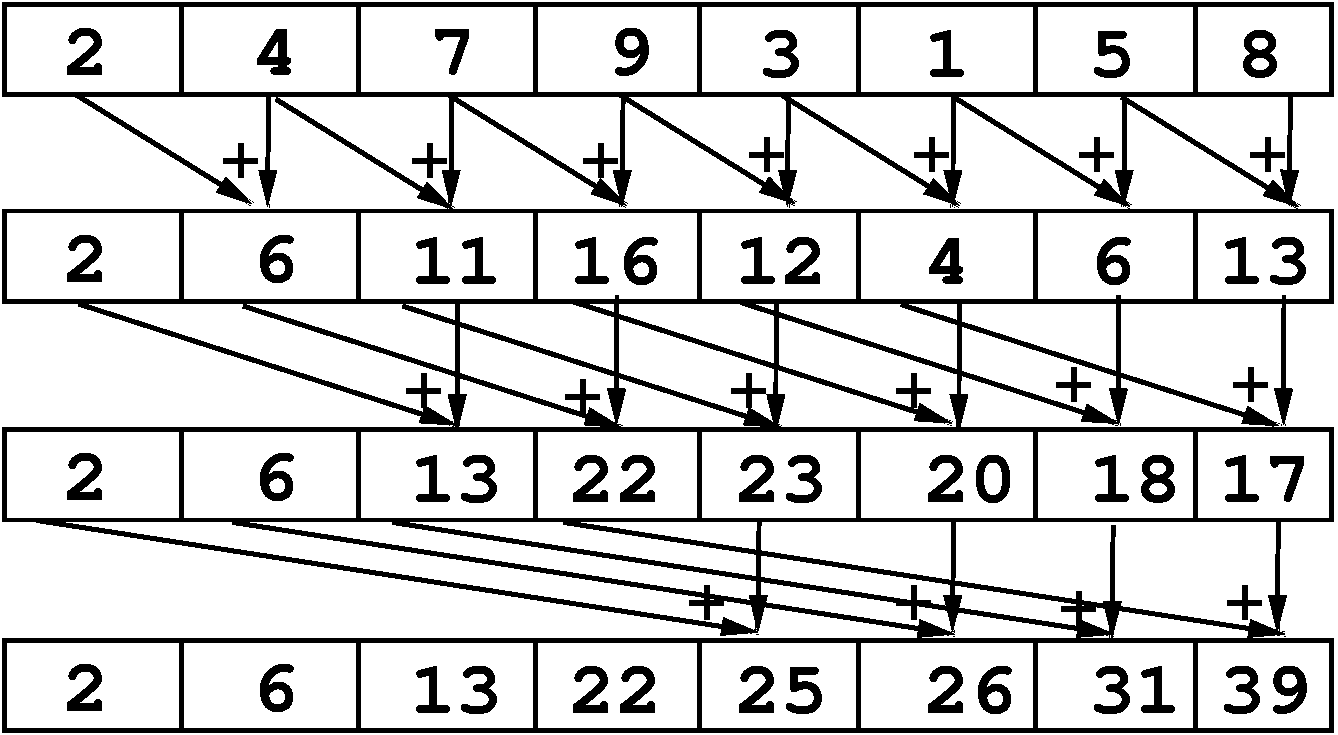
\includegraphics[height=30ex]{Figures/L2/SgmScanEg.pdf} 
\caption{Inclusive \lstinline{scan} used inside a warp for CUDA implementation.}
\label{fig:scan-eg-warp}
\end{figure} 

\begin{figure}
\begin{lstlisting}[mathescape=true]
Input:  array A of n=$2^k$ elements of type $\alpha$
        $\oplus$ : $\alpha\to\alpha\to\alpha$ associative
Output: B = [a$_1$, a$_1$$\oplus$a$_2$,$\ldots$,$\oplus_{j=0}^{n-1}$ a$_j$]
1.  forall i = 0 : n-1 do
2.    B[i] $\leftarrow$ A[i]
3.  endfor
4.  for d = 0 to k-1 do
5.    h = 2$^d$
6.    forall i = h to n-1 do 
7.      B[i] $\leftarrow$ B[i-h] $\oplus$ B[i]
8.    endfor
9.  endfor
\end{lstlisting}\vspace{-4ex}
\caption{Imperative Pseudcode for warp-level inclusive scan in CUDA; $n=32$}
\label{fig:warp-scan-inc}
\end{figure}

The pattern of a work-inefficient algorithm for inclusive scan is shown
in \cref{fig:scan-eg-warp}, and the pseudocode is presented in 
\cref{fig:warp-scan-inc}. This is the typical CUDA implementation
for a warp of threads---a warp is the unit of parallel execution
in CUDA and consists of $32$ consecutive threads.  Note that
the depth of the implementation is optimal: $D(n) = \Theta(lg \ n)$,
but the work is not:  $W(n) = \Theta(n~lg~n)$. However, on CUDA
platforms, any warp of threads executes in lock-step (in SIMD fashion), 
and de-selecting threads from execution (within one warp) brings no 
benefits. In fact this implementation is a factor of $2\times$ faster
than the one based on the up- and down-sweep, because it performs
only one sweep---its depth is $lg~n$ instead of $2~lg~n$. 

The remaining of this (sub)section discusses the \textbf{\em segmented scan} 
operator. A segmented scan semantically operates on an array of arrays---think 
a matrix in which the rows do not necessarily have the same length---and it
results in an array of arrays of similar shape as the input, in which each
of the resulted subarrays are obtained by scanning the corresponding input
subarray with the given associative binary operator (and neutral element).
Thus the semantics of a segmented scan is a map over the input array, in 
which the mapped function performs a scan on each subarray. The example
below demonstrates the semantics of an inclusive segmented scan:
\begin{lstlisting}[mathescape=true]
sgmScan (+) 0 [[1,3,5], [7,8], [9,11,14,15]] $\equiv$
[scan (+) 0 [1,3,5], scan (+) 0 [7,8], scan (+) 0 [9,11,14,15]] $\equiv$
[[1,4,9], [7,15], [9,20,34,49]]
\end{lstlisting}\vspace{-2ex}

The example above specifies the semantics but does not give insight into
what a data-parallel implementation should be. The major obstacle is that
the array of arrays is typically represented as an array of pointers,
each pointing to the corresponding subarray.
However this representation is not suitable for parallel execution: we 
need a flat data-structure! As such, we represent the array of arrays 
by a flat array of \emph{values}---whose length {\tt n} is the total
number of elements, i.e., the sum of the lengths of the subarrays---together 
with a \emph{flag} array, which has {\tt 1} (or \lstinline{true}) in the 
first position that starts a subarray, and {\tt 0} (or \lstinline{false}) 
in the remaining positions. One may also add to the representation a
shape array, which has number-of-subarrays integral elements, each
containing the lengths of its corresponding subarray. We present an 
example below that demonstrates the data-parallel representation 
(shape + flag + value flat arrays):
\begin{lstlisting}[mathescape=true]
nestedArray = [[1, 3, 5], [7, 8], [9, 11, 14, 15]]
   $\downarrow$            $\downarrow$          $\downarrow$        $\downarrow$
shapeArray  = [ 3,         2,      4             ]
flagArray   = [ 1, 0, 0,   1, 0,   1, 0,   0, 0  ]
valueArray  = [ 1, 3, 5,   7, 8,   9, 11, 14, 15 ]
\end{lstlisting}\vspace{-2ex}

It follows that the segmented scan has almost the same type as scan,
the only difference being that it receives one extra argument: the flag
array, which is represented as an array of booleans (or integers):
\begin{lstlisting}[mathescape=true]
sgmScan : ($\alpha\to\alpha\to\alpha$) $\to$ $\alpha$ $\to$ $\Pi$ n. [n]bool $\to$ [n]$\alpha$ $\to$ [n]$\alpha$
\end{lstlisting}\vspace{-2ex}
%We also note that the shape array is not necessary for the implementation
%of segmented scan.

\begin{figure}
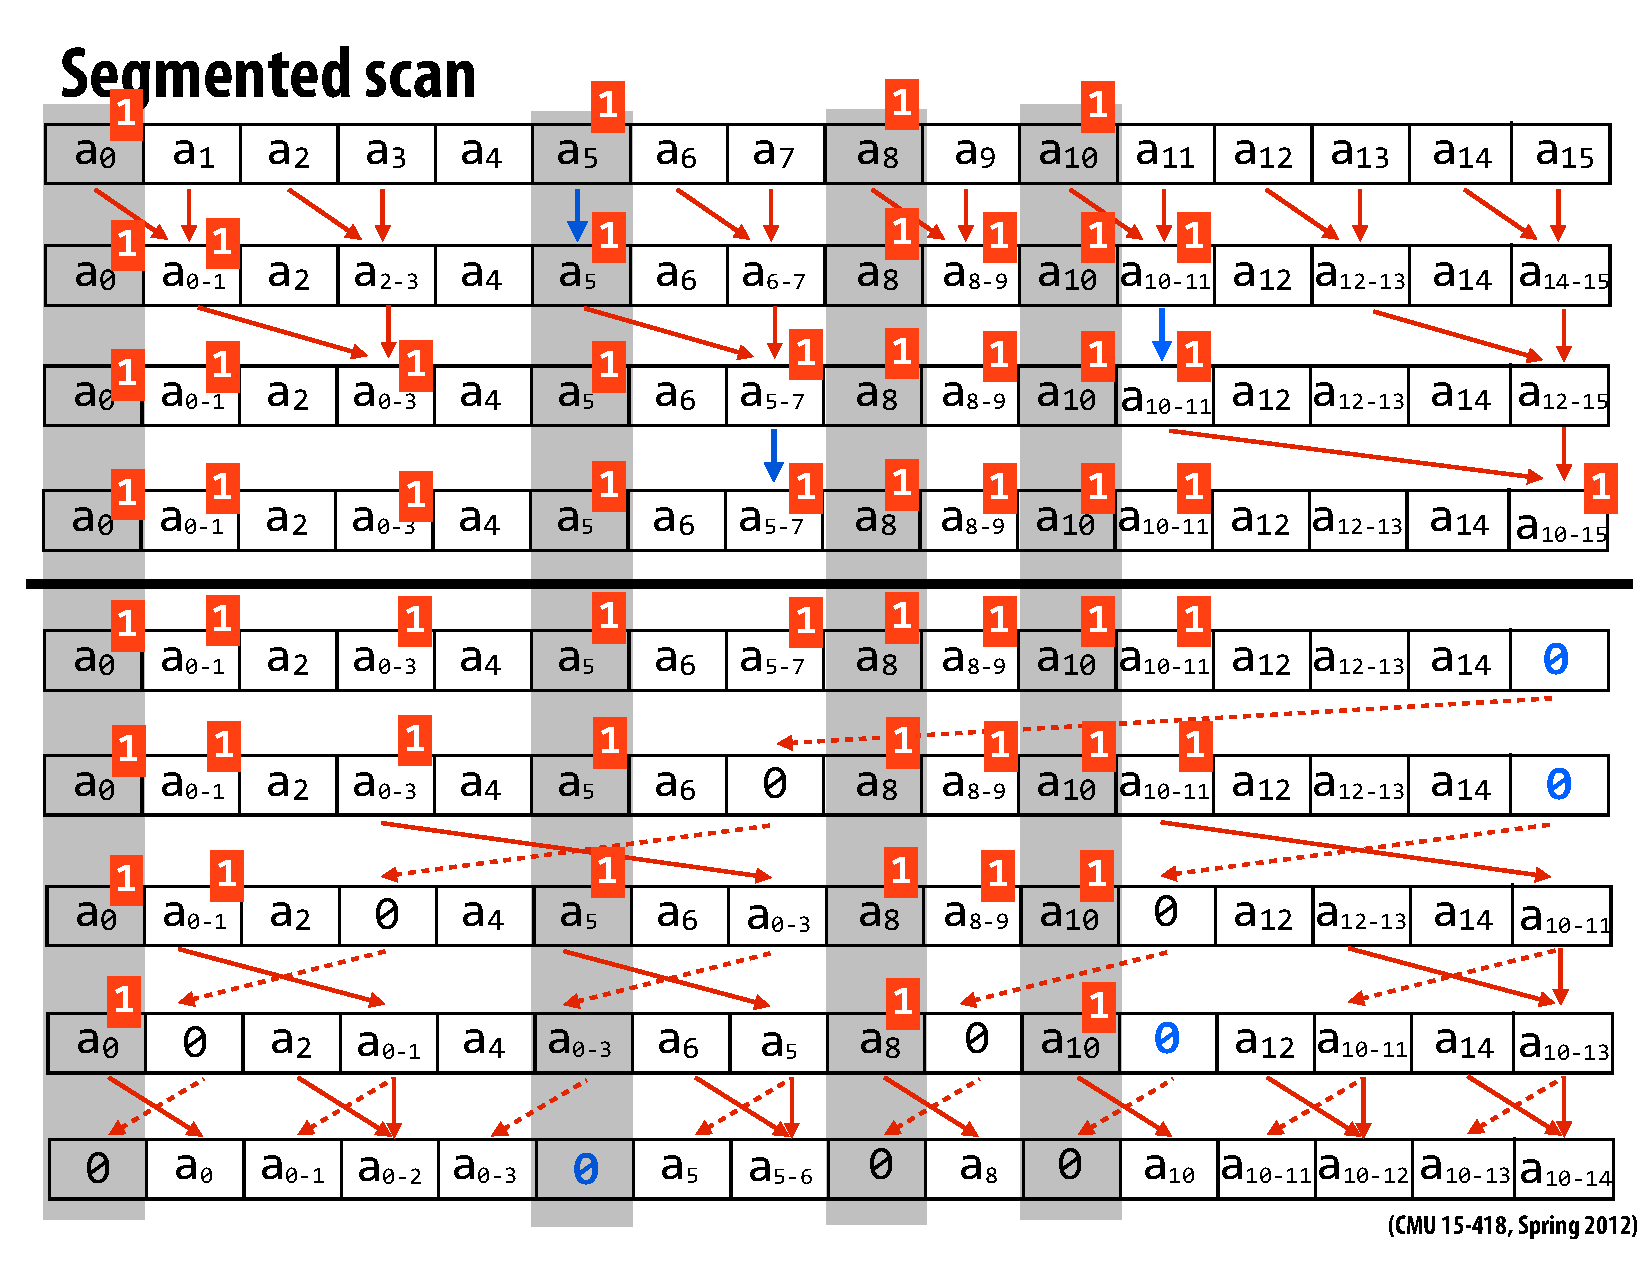
\includegraphics[height=55ex]{Figures/L2/Sgm-Excl-Scan-Eg.pdf} 
\caption{Parallel execution of exclusive segmented scan. Figure courtesy of CMU 15-418, Spring 2012}
\label{fig:sgm-scan-eg}
\end{figure} 

\begin{figure}
\begin{lstlisting}[mathescape=true]
Input:  flag array F of n=2$^k$ of ints/bools
        data array A of n=2$^k$ elements of type $\alpha$
        $\oplus$ : $\alpha\to\alpha\to\alpha$ associative
Output: B = segmented scan of 2-dimensional (irregular) array A
1.  forall i = 0 to n-1 do B[i] $\leftarrow$ A[i] endfor
2.  for d = 0 to k-1 do -- up-sweep pass
3.    forall i = 0 to n-1 by 2$^{d+1}$ do 
4.      if F[i+2$^{d+1}$-1] == 0 then 
5.          B[i+2$^{d+1}$-1] $\leftarrow$ B[i+2$^{d}$-1] $\oplus$ B[i+2$^{d+1}$-1]
6.      endif
7.      F[i+2$^{d+1}$-1] $\leftarrow$ F[i+2$^{d}$-1] .|. F[i+2$^{d+1}$-1] -- .|. is bitwise-or
8.  endfor endfor
9.  B[n-1] $\leftarrow$ 0
10. for d = k-1 downto 0 do -- down-sweep pass
11.   forall i = 0 to n-1 by 2$^{d+1}$ do 
12.     tmp $\leftarrow$ B[i+2$^{d}$-1]
13.     if F_original[i+2$^{d}$] $\neq$ 0 then
14.          B[i+2$^{d+1}$-1] $\leftarrow$ 0
15.     else if F[i+2$^{d}$-1] $\neq$ 0 then
16.          B[i+2$^{d+1}$-1] $\leftarrow$ tmp
17.     else B[i+2$^{d+1}$-1] $\leftarrow$ tmp $\oplus$ B[i+2$^{d+1}$-1]
18.     endif
19.     F[i+2$^{d+1}$-1] $\leftarrow$ 0
20. endfor endfor
\end{lstlisting}\vspace{-4ex}
\caption{Imperative Pseudcode for implementing exclusive segmented scan}
\label{fig:imperative-sgm-scan-exc}
\end{figure}



For completeness, \cref{fig:sgm-scan-eg} shows a graphical representation
of the execution pattern of exclusive segmented scan, and 
\cref{fig:imperative-sgm-scan-exc} shows the imperative pseudocode for
exclusive segmented scan. While there are more branches, it is relatively
straightforward to see that the depth and work asymptotics of segmented
scan remains the same as the one of scan: $D(n) ~=~ \Theta(lg~n)$ and
$W(n) ~=~ \Theta(n)$.   Understanding the execution pattern and pseudocode
is difficult: the teacher advices to {\em not} attempt it because
it does not really provide essential new insight. 

Instead, we make the \textbf{\em essential observation} that a segmented 
scan can be straightforwardly implemented in terms of a scan, which basically 
means that if an efficient implementation of scan is given, then we can 
directly derive an efficient implementation of segmented scan, and moreover,
that segmented scan has the same work and depth complexity as scan.


The code below shows the Futhark implementation of the inclusive segmented scan:
\begin{lstlisting}[mathescape=true]
let segmented_scan [n] 't (op: t -> t -> t) (ne: t)
                          (flags: [n]bool) (arr: [n]t): [n]t =
  let (_, res) = unzip <|
    scan (\(x_flag,x) (y_flag,y) -> -- extended binop is denoted $\odot$
             let fl = x_flag || y_flag
             let vl = if y_flag then y else x `op` y
             in  (fl, vl)
         ) (false, ne) (zip flags arr)
  in  res
\end{lstlisting}\vspace{-2ex}
The implementation consists of a \lstinline{scan} whose
input array is obtained by zipping the flag and value arrays, and
whose binary associative operator combines two flag-value tuples:
\begin{itemize}
    \item {\tt (x\_flag,x)} is the accumulator and {\tt (y\_flag,y)} 
        corresponds to the flag and value of the current element of 
        the input array;
    \item  the segmented-scan operator computes the resulting value
        by checking whether the current element corresponds to the start
        of a segment (i.e., tests whether {\tt y\_flag} is true).
        \begin{itemize}
            \item if this is the start of a segment, then
                the resulting value is the current element
                value ({\tt y}), as dictated by the semantics
                of inclusive segmented scan;
            \item otherwise we need to accumulate the current
                value: \lstinline{x `op` y}
        \end{itemize}
    \item the segmented-scan operator computes the resulting flag
        by taking the logical or of the two argument flags. This is
        necessary in order to propagate the start-of-a-segment flag,
        because parallel execution may proceed in a different order
        than the sequential execution. 
    \item We leave as exercised to verify that the scan's operator is 
        associative, i.e.,\\
        {\tt ((x\_flag,x) $\odot$ (y\_flag,y)) $\odot$ (z\_flag,z)} equals\\
        {\tt (x\_flag,x) $\odot$ ((y\_flag,y) $\odot$ (z\_flag,z))},
        and the check that the neutral element
        of the monoid induced by $\odot$ is indeed \lstinline{(false, ne)}.
\end{itemize}


\subsubsection{Implementation of Partition (Filter)}
\label{subsubsub:filter-impl}
$\mbox{ }$\\

We have already presented the type and semantics of \lstinline{filter}.
The question is: ``can filter be implemented in terms of \lstinline{map},
\lstinline{scan}, and \lstinline{scatter}?''
The answer is positive! 

In the following we will derive the implementation of a slightly more complicated 
construct than filter, named \lstinline{partition}, which has type:
\begin{lstlisting}[mathescape=true]
partition : ($\alpha~\to~$bool) $\to$ $\Pi$ n. [n]$\alpha$ $\to$ ([n]$\alpha$,i32) 
\end{lstlisting}\vspace{-2ex}
Partition is similar to \lstinline{filter}, in that it receives
as arguments a predicate and an input array, but it returns
an array of the same length as the input array and an integer.
The array result contains the same elements as the input array,
but in a different order: 
\begin{itemize}
    \item the elements that succeed under the predicate
            come before the ones that fail the predicate,
    \item the relative order of the elements in the two
            subarrays is the same as in the original array.
\end{itemize}
The scalar (integral) result is the number of elements that succeed 
under the predicate. 

\begin{figure}
\begin{lstlisting}[mathescape=true]
let partition2 [n] 't                    -- Assume t = i32, n = 6,
           (e: t) (p : (t -> bool))      -- p (x:i32)= 0 == (x%2),
           (arr : [n]t) : ([n]t, i32) =  -- arr = [5,4,2,3,7,8]
  let cs  = map p arr                    -- cs  = [F,T,T,F,F,T]
  let tfs = map (\f -> if f then 1       -- tfs = [0,1,1,0,0,1]
                            else 0) cs
  let isT = scan (+) 0 tfs               -- isT = [0,1,2,2,2,3]
  let i   = isT[n-1]                     -- i   = 3

  let ffs = map (\f->if f then 0 
                          else 1) cs     -- ffs = [1,0,0,1,1,0]
  let isF = map (+i) <| scan (+) 0 ffs   -- isF = [4,4,4,5,6,6]
  let inds= map3 (\c iT iF ->            -- inds= [3,0,1,4,5,2]
                    if c then iT-1 
                         else iF-1
                 ) cs isT isF
  let r = scatter (replicate n e) inds arr -- r = [4,2,8,5,3,7]            
  in  (r, i) 
\end{lstlisting}\vspace{-4ex}
\caption{Implementation of a two-way partition in Futhark.}
\label{fig:futhark-partition2}
\end{figure}

The Futhark implementation is shown in \cref{fig:futhark-partition2};
we have added as first parameter a dummy value of the element type
of the array, which will be used to initialize an array that will
be subject to a parallel write (\lstinline{scatter} operator).
%
The right hand  side of \cref{fig:futhark-partition2} demonstrates
the code on an example. The implementation proceeds as follows:
\begin{itemize}
    \item First, the predicate is mapped on the input array,
            and the result is turned into ones (for \lstinline{true})
            or zeros (for \lstinline{false}), which are stored in
            array {\tt tfs}.
    \item An inclusive scan with addition is performed on {\tt tfs}
            resulting in array {\tt isT}. Please observe that 
            array {\tt isT} now holds the value of the indices at 
            which the elements that succeed under the predicate
            should appear in the result array (plus one). Also
            the last element of {\tt isT}, saved under variable 
            {\tt i} is the number of elements that succeed under 
            the predicate.
    \item Array {\tt isF} is computed in a similar fashion and
            holds the value of the indices at which the elements 
            that fail under the predicate
            should appear in the result array (plus one).
    \item The two pieces of information are combined together
            in array {\tt inds} from arrays {\tt isT} and {\tt isF}
            (and {\tt cs}) by means of a \lstinline{map3} operator.
    \item Finally, the \lstinline{scatter} operator is used to
            permute the array by {\tt inds}, and the result is
            written in a new array created by \lstinline{replicate}.
    \item The result is the permuted array, tupled with integer {\tt i},
            which denotes the number of elements that have succeed 
            under the predicate.
\end{itemize}


\subsubsection{Sparse-Matrix Vector Multiplication}
\label{subsubsub:sparse-mat-vec-mult}
$\mbox{ }$\\

\begin{figure}
\begin{lstlisting}[mathescape=true]
-- (a) Dense-Matrix Representation
[ [ 2.0, -1.0,  0.0, 0.0]              
, [-1.0,  2.0, -1.0, 0.0]
, [ 0.0, -1.0,  2.0,-1.0]
, [ 0.0,  0.0, -1.0, 2.0]
, [ 0.0,  0.0,  0.0, 3.0]
]

-- (b) Sparse Matrix represented as 
-- an array of pointers; each non-0 element 
-- records its value and column number:
[ [(0,2.0),  (1,-1.0)],
, [(0,-1.0), (1, 2.0), (2,-1.0)]
, [(1,-1.0), (2, 2.0), (3,-1.0)]
, [(2,-1.0), (3, 2.0)]
, [(3,3.0)]
]

-- (c) Flat Representation of Sparse Matrix:
shape = [2, 3, 3, 2, 1] -- number of non-0 elements of each row
flag  = [1, 0, 1, 0, 0, 1, 0, 0, 1, 0, 1]
value = [ (0,2.0), (1,-1.0), (0,-1.0), (1, 2.0), (2,-1.0),
          (1,-1.0), (2,2.0), (3,-1.0), (2,-1.0), (3,2.0), (3,3.0)]
\end{lstlisting}\vspace{-4ex}
\caption{ Matrix representations: (a) dense, (b) sparse array of pointers, (c) sparse flat.}
\label{fig:mat-reps}
\end{figure}

% x = [2.0, 1.0, 0.0, 3.0]

Figure~\ref{fig:mat-reps} shows several matrix representations
of a {\tt m$\times$n} matrix (where {\tt m=5} and {\tt n=4}):
\begin{itemize}
    \item[(a)] the dense representation is a two-dimensional
        array of type \lstinline{[m][n]f32}. Since the $2$-D array
        is regular---all rows have the same length---the array is 
        assumed to be stored contiguously in a memory space of
        size {\tt n$\times$m$\times$sizeof(f32)}.
    \item[(b)] the array-of-pointers sparse representation maintains
        pointers to the subarrays that represent the rows of the array,
        except that a row is represented only by the non-zero elements
        tupled with their corresponding column-number. Please note
        that now the array is irregular, since the number of non-zero
        element is not the same across all rows. 
    \item[(c)] the flat sparse representation corresponds to a triplet
        of shape, flag and value arrays. The shape array has size {\tt m}
        and holds the the number of non-zero elements on each row. The
        flag and value arrays are unidimensional (flat) and their length
        is equal to the total number of non-zero elements of the matrix.
        The latter are stored in the value array, while the flag array
        records a zero at the index of each element that starts a row.
        This is known as the CSR format.
\end{itemize}

Futhark supports only regular arrays---i.e., all rows of a matrix have 
the same length---hence it does not support arrays of pointers. 
However, assuming a language that supports arrays of pointers 
(such as Haskell), sparse matrix vector multiplication can be 
elegantly written using format (b) in the following Futhark-like 
pseudocode:
\begin{lstlisting}[mathescape=true]
let spMatVctMul [m][n] (mat: [m][](i32,f32)) (vct: [n]) : [m]f32 =
    map (\row -> let ps = map (\(i,v) -> v * vct[i]) row
                 in  reduce (+) 0.0f32 ps 
        ) mat
\end{lstlisting}\vspace{-2ex}
Please note that the implementation exhibits irregular parallelism:
the size of the inner \lstinline{map-reduce} operations differs 
across iterations of the outer \lstinline{map}. We will see later,
in \cref{sec:flattening} how to re-write this irregular nested
parallelism by means of (1) a flat-sparse-data representation 
in format (c), and (2) flat-parallel constructs (that do not exhibit
inner parallelism).

%\begin{figure}
%\begin{lstlisting}[mathescape=true]
%let spMatVctMul [m][n][q] (shp: [m]i32) (flgs: [q]bool) 
%                          (vals: [q](i32,f32)) (vct: [n]) : [m]f32 =
%  let shp_scn = scan (+) 0 shp
%  let shp_off = map (\k -> if k > 0 then shp_scn[k-1] else 0) shp_scn
%  in  map2 (\len off -> 
%                 let ps = map2 (\j -> let (v,i) = vals[off + j] 
%                                      in  v * vct[i]
%                               ) (iota len)
%                 in  reduce (+) 0.0f32 ps 
%          ) shp shp_off
%\end{lstlisting}\vspace{-4ex}
%\caption{ Sparse Matrix-Vector Multiplication: Flat Data and Nested Parallelism}
%\label{fig:spmv-flat-data-nest-par}
%\end{figure}
%
%For the moment, we aim to flatten the data, without keeping the nested
%parallelism. The question is: ``how do we rewrite this code to use the 
%(c) format of (flat-sparse) matrix representation?''. This is a necessary
%step in our ultimate goal of also flattening parallelism.   
%Figure~\ref{fig-nest-par-flat-rep} provides the answer to the question:
%\begin{itemize}
%    \item
%\end{itemize} 
%% 

\subsubsection{Prime Number Computation (Sieve)}
\label{subsubsub:primes}
$\mbox{ }$\\

This section discusses several implementations that, given
an integer {\tt n}, compute all the prime natural numbers 
less than or equal to {\tt n}. This example was introduced
in the well-known article ``Scan as Primitive Parallel 
Operation''~\cite{segScan}.

\begin{figure}
\begin{lstlisting}[mathescape=true]
int res[n+1] = [0, 0, 1, 1, 1, ..., 1]
for(i = 2; i <= sqrt(n); i++)
    if ( res[i] != 0 )
        forall m $\in$ multiples of i $\leq$ n} do
             res[m] = 0;
        endfor
    endif
endfor
\end{lstlisting}\vspace{-4ex}
\caption{Imperative pseudocode for the naive version of primes:
         Work $O(n \ lg \ lg \ n)$, Suboptimal Depth: $O(\sqrt{n})$. }
\label{fig:primes-naive-Imp}
\end{figure}

\medskip

The first implementation, shown in \cref{fig:primes-naive-Imp}, starts 
with an array {\tt res} of size {\tt n+1}, in which elements at 
indices $0$ and $1$ are zero, and the rest of the elements are ones. 
The meaning is that initially, all natural number greater than $1$ 
are considered prime numbers.
Then the implementation iteratively zeros out the array indices 
corresponding to all multiples of numbers less than or equal to $\sqrt{n}$.
This step is accomplished in parallel by means of the \lstinline{forall}
construct.   After the sequential loop terminates, the prime numbers
are the indices of {\tt res} that hold non-zero (one) values.

This (first) implementation has optimal work $O(n \ lg \ lg \ n)$ 
but suboptimal depth: $O(\sqrt{n})$. The latter can be easily observed:
the outer loop iterates sequentially to $\sqrt{n}-1$ times. We will
can this the naive implementation due to depth sub-optimality.

\begin{figure}
\begin{lstlisting}[mathescape=true]
-- Primes: Naive Version (primes-naive.fut)
-- ==
-- compiled input { 30 } output { [2,3,5,7,11,13,17,19,23,29] }
let main (n : i32) : []i32 =           -- Assume n = 9, sq = 3 
  let a  = map (\i -> if i==0 || i==1  -- a = [0,0,1,1,1,1,1,1,1,1]
                      then 0 else 1
               ) (iota (n+1))          -- iteration j=0, i=2, m=3
  let sq = t32 (f32.sqrt (r32 n))      -- inds = [4, 6, 8]
  let fl =                             -- vals = [0, 0, 0]
    loop(a) for j < (sq-1) do          -- a'= [0,0,1,1,0,1,0,1,0,1]
      let i    = j + 2
      let m    = (n / i) - 1           -- iteration j=1, i=3, m=2
      let inds = map (\k -> (k+2)*i)   -- inds = [6,9], vals = [0,0]
                     (iota m)          -- a'= [0,0,1,1,0,1,0,1,0,0]
      let vals = replicate m 0         
      let a'   = scatter a inds vals   -- iteration j=2, i=4, m=1
      in  a'                           -- a' unchanged
  in  filter (\i -> unsafe fl[i]!=0)   
             (iota (n+1))              -- Result: [2,3,5,7]
\end{lstlisting}\vspace{-4ex}
\caption{Futhark code for the naive version of primes:
            Optimal Work $O(n \ lg \ lg \ n)$, Suboptimal Depth: $O(\sqrt{n})$.}
\label{fig:primes-naive-Futhark}
\end{figure}

\medskip

The complete Futhark code for the naive version is shown in 
\cref{fig:primes-naive-Futhark}; it faithfully implements the
imperative pseudocode. Furthermore, the right-hand side of
the figure demonstrates the case for {\tt n=9}. Please note 
that the parallel \lstinline{forall} loop has be implemented
as a composition between \lstinline{scatter} and \lstinline{map}.
This is fused by the Futhark compiler, so the generated code
is as efficient as the imperative one. 

\bigskip

The naive version of primes is a good starting point, but we
are unhappy with the fact that the depth is simply too high 
$O(\sqrt{n})$.
%
Luckily, the solution is not terribly complicated: One can
reason that if the primes $p$ between $2$ and $\sqrt{n}$ are 
known (and stored in array {\tt sqrn\_primes}), then we could 
generate all multiples of those primes at once.
In the data parallel language NESL, which supports irregular
nested parallelism, this computation could be expressed by 
means of the array comprehension
{\tt \{[2*p : n : p] : p in sqrn\_primes\}} which semantically
results in an array of arrays, in which each subarray
corresponds to one of the known prime numbers between
$2$ and $\sqrt{n}$. For a given {\tt p}, its subarray
consists of the elements {\tt [2*p, 3*p, 4*p, $\ldots$]}
which are less than or equal to {\tt n}, i.e., the slice that
starts from {\tt 2*p} and goes with a stride equal to 
{\tt p}.

\begin{figure}
\begin{lstlisting}[mathescape=true]
let main (n : i32) : []i32 =
  let sqrn_primes   = [2]
  let len  = 2
  let (sqrn_primes,_) =
    loop (sqrn_primes, len) while len < n do
      -- this is "len = min n (len*len)"
      let len = if n / len < len then n else len*len

      let composite = -- uses nested parallelism
            map (\p -> let m   = len / p
                       let arr = map (+2) (iota (m-1))
                       in  map (*p) arr
                ) sqrn_primes
      let not_primes = reduce (++) [] composite -- flattens data

      let flat_size  = length not_primes
      let zero_array = replicate flat_size false
      let mostly_ones= map (> 1) (iota (len+1))
      let prime_flags= scatter mostly_ones not_primes zero_array
      let sqrn_primes= filter (\i-> i>1 && i<=n && prime_flags[i])
                              (iota (len+1))
      in  (sqrn_primes, len)
  in sqrn_primes
\end{lstlisting}\vspace{-4ex}
\caption{Futhark-like (illegal) nested-parallel code for primes:
            Optimal Work $O(n~lg~lg~n)$ and Depth: $O(lg~lg~n)$.}
\label{fig:primes-nested-par-Futhark}
\end{figure}

A Futhark-like pseudocode is shown in 
\cref{fig:primes-nested-par-Futhark}---please remember that
Futhark does not support irregular arrays/parallelism, so 
this implementation would not even compile with Futhark; we
just use it for consistency.  The implementation starts with
a known set of primes {\tt [2]} less than or equal to {\tt len=2}.
Each iteration of the loop computes a new set of primes
less than or equal to {\tt len$^2$} (for simplicity):
\begin{itemize}
    \item The {\tt composite} array is computed by means of 
        nested-parallelism and it contains all the multiples 
        of the currently known set of primes. The code is 
        semantically equivalent to the previously-discussed 
        NESL array comprehension:
        {\tt \{[2*p : n : p] : p in sqrn\_primes\}}.
    \item The {\tt not\_primes} array is the flattened version
        of {\tt composite}, which is an array of arrays.
    \item The {\tt prime\_flags} array is computed by
        a \lstinline{scatter} operator that 
        \begin{itemize}
            \item writes into an array of mostly one (true) values
            \item at the indices corresponding to the computed 
                    multiples of prime numbers
            \item the zero (false) values in order to indicate
                    that those positions do {\em not} correspond
                    to prime numbers.
        \end{itemize}
    \item the \lstinline{filter} operator extracts the indices
            that correspond to prime numbers (true/one values).
\end{itemize}

We will not demonstrate how the nested parallel implementation
works on a simple example in which {\tt n} is $9$. 
Initially, {\tt len=2} and {\tt sqrn\_primes = [2]}.
In the first iteration of the loop: {\tt len} is set to $2^2 = 4$,
and {\tt composite = [[2*2]] = [[4]]} because there is only
one prime {\tt p=2} for which {\tt m=4/2=2} and {\tt arr = [2]}.
As such \lstinline{prime_flags = scatter [0,0,1,1,1] [4] [0] = [0,0,1,1,0]}
and the result of the filter is thus {\tt [2,3]}---the set of 
primes to be used for the next iteration.

The second iteration initially has {\tt len=4} and 
{\tt sqrn\_primes = [2,3]}. Then {\tt len} is set to {\tt 9}.
Since there are two primes {\tt 2} and {\tt 3}, the
{\tt composite} array is computed as {\tt [[4,6,8],[6,9]]},
where the first subarray corresponds to {\tt p=2} and {\tt m=9/2=4}
and the second subarray corresponds to {\tt p=3} and {\tt m=9/3=3}.
It follows that {\tt not\_primes = [4,6,8,6,9]} and
{\tt prime\_flags} is computed as\\
\lstinline{scatter [0,0,1,1,1,1,1,1,1] [4,6,8,6,9] [0,0,0,0,0]}\\
which results in {\tt [0,0,1,1,0,1,0,1,0,0]}, hence the
primes less than or equal to $9$ are extracted by the
\lstinline{filter} operation as: {\tt[2,3,5,7]}.

\medskip

It remains now to verify that this implementation has improved the
depth and by how much.
The depth corresponds to the count of the sequential 
loop---meaning we need to answer the question: ``how many iterations
does the sequential loop has?''   One can observe that {\tt len} 
starts at $2=2^{2^0}$ and each iteration squares up the value of {\tt len}:
in the first iteration {\tt len} is $2^{2^1}$, in the second is $(2^2)^2=2^{2^2}$,
in the third is $(2^4)^2=2^8=2^{2^3}$, hence one can easily
prove by induction that in some iteration $k$ the value of {\tt len} 
is $2^{2^k}$.
It follows that the total number of iterations of the loop
is the first $k$ such that $2^{2^k} \geq n$, hence the depth of 
the new nested-parallel version is $O(lg~lg~n)$.


\subsubsection{Quicksort}
\label{subsubsub:quicksort}
$\mbox{ }$\\

\begin{figure}
\begin{lstlisting}[mathescape=true]
isSorted [n] (arr: [n]i32) : bool =
  reduce (&&) true <|
  map (\i -> i == 0 || arr[i-1] <= arr[i]) (iota n)

nestedQuicksort [n] (arr: [n]i32) : [n]i32 = 
  if n <= 1 || isSorted arr then arr
  else
  let i  = getRand (0, (length arr) - 1)
  let a  = arr[i]
  let s1 = filter (\x -> (x <  a)) arr
  let s2 = filter (\x -> (x >= a)) arr
  let rs = map nestedQuicksort [s1, s2]
  in  (rs[0]) ++ (rs[1])
\end{lstlisting}\vspace{-4ex}
\caption{Futhark-like nested-parallel code for quicksort. (Please be aware that this code is illegal in Futhark!)}
\label{fig:quicksort-nested-par-Futhark}
\end{figure}

A Futhark-like nested-parallel pseudocode for quicksort is shown in 
Figure~\ref{fig:quicksort-nested-par-Futhark}:
\begin{itemize}
    \item Please note that this is illegal Futhark code, that will
        fail compilation because of two reasons: (1) Futhark does
        not support recursion and (2) the array {\tt [s1,s2]} passed 
        to the recursive call is irregular---the two subarrays do not
        necessarily have the same length.
    \item The implementation picks a random pivot {\tt a} and uses the
        \lstinline{filter} operator to split the array into two subarrays:
        one containing the elements less than the pivot and one containing 
        the other elements.
    \item The two subarrays are recursively processed (sorted) by the recursive
        call\\ \lstinline{map nestedQuicksort [s1, s2]} and the sorted results
        are concatenated together to form the sorted array. (The partitioning
        has already ensured that all the elements of the first subarray are 
        necessarily smaller than the ones of the second.) 
        Please note that the call \lstinline{map nestedQuicksort [s1, s2]}
        gives raise to nested parallelism: the divide-and-conquer nature
        gives raise to a tree in which, in principle, \lstinline{filter}
        operations can be applied in parallel on all the nodes at the same 
        breadth level in the tree.
    \item The recursion terminates when the length of the list is less than
        or equal to $1$---a one-element list is always sorted---or when the
        array is already sorted. The latter is checked with the {\tt isSorted}
        function, which is implemented by means of a \lstinline{map-reduce}
        composition.   
    \item Please note that the use of {\tt isSorted} is not
        an optimization; it is actually necessary to ensure termination. 
        A typical quicksort implementation would perform a three-way partitioning
        of the array: the elements less than, equal to and greater than the pivot.
        For simplicity, the presented implementation uses a two-way partition,
        but this may end up with an array of length $>1$ containing the same
        element, which makes the sorted condition necessary.
    \item Finally, the three-way splitting version has average work complexity
        $n ~lg~n$ and average depth $lg~n$. The later assumes that \lstinline{filter}
        has depth $O(1)$; in practice the average depth complexity is $lg^2~n$.
\end{itemize}

We conclude by demonstrating quicksort's execution on the simple example when
the input array is {\tt arr = [3,2,4,1]}. 
Assume random {\tt i = 0}, hence {\tt a = 3}. It follows that the array is 
partitioned into two subarrays, one {\tt s1 = [2,1]} which has elements less 
than {\tt 3}, and the other {\tt s2 = [3,4]} which has its elements greater
or equal to three. Next quicksort is (mapped) performed on the two subarrays.

In the case of {\tt nestedQuicksort [2,1]}, assume we pick {\tt i=0}, leading
to {\tt a = 2} and we partition {\tt [2,1]} into subarrays {\tt [1]} and {\tt [2]}.
These are recursively processed but they hit the base-case since they have length
equal to $1$, hence they are returned without modification and concatenated into
sorted array {\tt [1,2]}.

The case of {\tt nestedQuicksort [3,4]} hits the base case, since it succeeds
under the {\tt isSorted} predicate.

The final step is to concatenate the results of the two calls to {\tt nestedQuicksort},
resulting in sorted array {\tt [1,2] ++ [3,4] = [1,2,3,4]}!

\newpage
\section{Flattening Transformation}
\label{sec:flattening}

We have seen in the previous section how non-trivial applications
can be naturally constructed by combining parallel operators at the
same level or at different levels in a parallel nest. We have also
seen that nested parallelism allows to reason asymptotically about 
the parallel behavior of the implementation, such as its work and 
depth. 

However exploiting nested parallelism is notoriously difficult.
Direct utilization of nested parallelism may be possible on some
hardware, such as CPU. For example the parallelism of quicksort
can be exploited by \emph{dynamically} spawning threads at each
divide and conquer step. This technique however is not guaranteed
to result in good performance, for example because the distribution
of work across threads may be very unbalanced.

More important, a big class of highly-parallel hardware, such as
GPUs support only very limited forms of recursion and dynamic
parallelism, if at all! Morally, the hyardware execution is organized 
on one (or maybe two) flat-parallel levels---for example, on GPUs 
one typically exploits grid-level parallelism, and occasionally
block-level parallelism, which allows threads within a block-group
to communicate by means of shared (scratchpad) memory. This means
that direct mapping of application parallelism will require a choice
of which level to parallelize and which to sequentialize, because 
it is not directly-possible to parallelize both levels. 

It follows that there is a big disconnect between the nested-parallel
form of the program---which has the advantage that it resembles well
the algorithmic specification---and a semantically equivalent form
of the program that can be efficiently and statically mapped (executed) 
on highly-parallel hardware. The latter form might be efficient to
execute, but likely it resembles little the original algorithm and
causes modularity and maintainability issues. Ideally, the re-writing
should be done automatically by the compiler, thus getting the best
of the two worlds. 

This section presents the intuition behind the seminal work on the
NESL data-parallel language~\cite{BlellochCACM96NESL} related to
the flattening transformation~\cite{blelloch1994implementation}
that
\begin{itemize}
    \item \emph{statically} transforms an arbitrarily-nested data-parallel 
        program into a semantically equivalent one that uses only 
        flat-parallel construct (no nesting of parallelism), 
    \item in a way that preserves the work and depth asymptotic
        of the original nested-parallel program.
\end{itemize}

The flattening transformation does not (completely) solve the problem, 
for example because it requires high memory usage and does not
account for communication costs; in fact it often prevents 
opportunities for locality optimizations, because of excessive
utilization of parallelism in excess of what the hardware can 
support.\footnote{Various efforts have focused on addressing these issues by 
restricting flattening in various ways, for example by flattening 
only the data and leaving the nested-parallel structure 
intact~\cite{Bergstrom:2013:DFN:2442516.2442525},
by applying flattening at the granularity of the largest sequential
subexpression~\cite{Keller:2012:VA:2364506.2364512}, by aggressive
fusion of segmented operations enabled by shape analysis~\cite{nessie:cpc15},
or by mechanisms for streaming irregular 
arrays~\cite{madsen2016streaming,AccelerateStreaming} that optimize
memory footprint. NESL has also been implemented on GPU 
hardware~\cite{Bergstrom:2012:NDG:2398856.2364563}.} 

\textbf{\em However, what flattening primarily offers is a systematic way 
of reasoning about and transforming nested parallelism. The goal of this 
chapter is} not necessarily to formally introduce the flattening 
transformation, but instead \textbf{\em to acquire a deep-enough feeling 
of how it works}. The intent is to train you by means of practical 
examples, so that you will acquire a sufficient understanding that would 
allow you to apply its principles in future practical work related to 
GPU parallelization (or other highly-parallel hardware).  

This section is organized as follows:
\begin{itemize}
    \item \cref{subsec:flatten-rules} presents an incomplete set of 
        rules related to the flattening of specific code patterns.
    \item \cref{subsec:flatten-simple-eg} demonstrates how the 
        previously-discussed rules can be combined to flatten a 
        trivial program.
    \item \cref{subsec:flat-exercises} advises on how to start
        reasoning about flattening the nested-parallel versions
        of sparse-matrix vector multiplication, prime-number computation,
        and quicksort. These applications were introduced in
        sections~\ref{subsubsub:sparse-mat-vec-mult},~\ref{subsubsub:primes}~and~\ref{subsubsub:quicksort},
        respectively. The first two are weekly-assignment tasks,
        and the latter may be a group project.
\end{itemize}

\subsection{Rules For Flattening}
\label{subsec:flatten-rules}

We present first the intuition behind the flat-data representation
(\cref{subsubsec:data-flat}), then we present the rules for flattening
several constructs which are directly nested inside a map:
scan, map, replicate, iota, if-then-else expressions, and reduce. 

\subsubsection{Data Flattening}
\label{subsubsec:data-flat}
$\mbox{ }$\\

A two-dimensional irregular array---think array of pointers or 
list of lists---can be represented in a flat way by means of
a shape array and a data array, which are both unidimensional
arrays that have contiguous support in memory and hence are
suitable for data-parallel programming. 

For example, the list of lists:
{\tt aoa = [[a$^{1}_{1}$,$\ldots$, a$^{1}_{m{_1}}$],$\ldots$, [a$^{r}_{1}$,$\ldots$, a$^{r}_{m{_r}}$]]}
can be represented 
\begin{itemize}
    \item[(1)] by the shape array {\tt aoa\_shp = [m$_1$,$\ldots$, m$_r$]}, which specifies the length
            of each sublist, and
    \item[(2)] by the flat-data array
    {\tt aoa\_val = [a$^{1}_{1}$,$\ldots$, a$^{1}_{m{_1}}$, $\ldots$, a$^{r}_{1}$,$\ldots$, a$^{r}_{m{_r}}$]}.
\end{itemize}

\begin{figure}
\begin{lstlisting}[mathescape=true]
mkFlagArray [m] (aoa_shp: [m]i32) : []i32 = -- aoa_shp = [3,1,4,2]
  let shp_scn = scan (+) 0 aoa_shp          -- shp_scn = [3,4,8,10]
  let aoa_len = shp_ind[m-1]                -- aoa_len = 10
  let shp_ind =                             -- shp_ind = [0,3,4,8]
    map (\i -> if i==0 then 0     -- scatter [0,0,0,0,0,0,0,0,0,0]
               else shp_ind[i-1]  --         [0,3,4,8]
        ) (iota m)                --         [1,1,1,1]
  in scatter (replicate aoa_len 0)--------------------------------
             shp_inds (replicate m 1)-- res= [1,0,0,1,1,0,0,0,1,0] 
\end{lstlisting}\vspace{-4ex}
\caption{Constructing the flag array from the shape array}
\label{fig:make-flag}
\end{figure}

However, we have seen that a segmented scan operator requires
a flag array: semantically an array of ones and zeros (booleans),  
which has the same size as the data array, and which records with
a one (true) the element that starts a (new) subarray and zero (false)
otherwise. The question is ``how do we construct the flag array from
the shape array''?  \cref{fig:make-flag} provides the implementation
together with a side example:
\begin{itemize}
    \item[(a)] first the shape array is scanned with addition and 
        the result is recorded in {\tt shp\_scn};
    \item[(b)] the length of the flag/data array is the last element
            of {\tt shp\_scn};
    \item[(c)] {\tt shp\_scn} is semantically rotated/shifted-right
            by one element resulting in array {\tt shp\_ind},
            which contains the positions that start a subarray
            in the flat data/flag representation;
    \item[(d)] a \lstinline{scatter} writes into an array of zeroes,
            the value one at the positions recorded in {\tt shp\_ind};
            this creates the flag array, denoted by {\tt aoa\_flg}.
    \item[(e)] sometimes it is useful to have the flag array
            recording the start of each subarray by its size,
            rather than by a one. This can be easily accomplished
            by changing the result expression to:\\
            \lstinline{scatter (replicate aoa_len 0) shp_inds aoa_shp},
            which results in the flag array\\
            {\tt[3,0,0,1,4,0,0,0,2,0]}.
\end{itemize}

Next, we will play with distributed various information
to each member of the data array:
\begin{itemize}
    \item[(f)] ``How can we record for each
                 data member the size of its corresponding subarray?''\\
                With our example the result we seek would be
                {\tt[3,3,3,1,4,4,4,4,2,2]}. This can be simply
                accomplished by a segmented inclusive scan with addition
                on the format (e) of the flag array, i.e.,
                \lstinline{sgmScan (+) 0 aoa_flg aoa_flg}.
   \item[(g)] ``How can we record for each
                 data member the index of its corresponding subarray?''\\
                With our example the result we seek would be
                {\tt[0,0,0,1,2,2,2,2,3,3]}. This can be simply
                accomplished by scanning with addition the
                one-and-zero representation of the flag array
                and then subtracting one from each element of
                the result, i.e., 
                \lstinline{map (-1) <| scan (+) 0 aoa_flg}
\end{itemize}

While we will mostly work with two-dimensional irregular arrays, 
we conclude this section by reasoning about how to generalize 
the flat representation for a $k$-dimensional array. This 
can be simply achieved by recording $k-1$ shape arrays,
i.e., one for each outer dimension.
For example, the three-dimensional array
{\tt [ [[1,2,3], [4,5], [6,7]], [[9], [8,7], [6], [5,4,3,2]] ]}
is represented by the the shape arrays {\tt aoa\_shp0} and
{\tt aoa\_shp1} and by the flat-data array {\tt aoa\_val}:
\begin{lstlisting}[mathescape=true]
aoa_shp0 = [3, 4]
aoa_shp1 = [3,2,2,1,2,1,4]
aoa\_val = [1,2,3,4,5,6,7,9,8,7,6,5,4,3,2]
\end{lstlisting}\vspace{-2ex}
If required, we can create flag arrays for each dimension,
for example from {\tt aoa\_shp0} one can compute
{\tt aoa\_flg0 = [1,0,0,1,0,0,0]} and from {\tt aoa\_shp1}
one can compute {\tt aoa\_flg1 = [1,0,0,1,0,1,0,1,1,0,1,1,0,0,0]},
by using the {\tt mkFlagArray} function shown in \cref{fig:make-flag}.
Furthermore, one can distribute various information across the 
data elements of the arrays in a similar fashion with the one 
used for the two-dimensional arrays.


\subsubsection{Flattening a Scan Directly Nested in a Map}
\label{subsubsec:scna-in-map} 




\subsection{Flattening a Simple, Contrived Program}
\label{subsec:flatten-simple-eg}


\subsection{Flattening Exercises}
\label{subsec:flat-exercises}



\newpage
%% Bibliography
\bibliography{pmph.bib}

\end{document}

%%% Local Variables:
%%% mode: latex
%%% TeX-master: t
%%% End:
